%\documentclass[10pt, conference, compsocconf]{IEEEtran}
%\IEEEoverridecommandlockouts
%
% $Header: http://maccattaneo:8081/svn/Cattaneo/Articoli/SEESMS/SEESMS_journal.tex 133 2011-07-20 18:17:11Z cattaneo $
%

\documentclass[authoryear]{elsarticle}
%\documentclass[preprint]{elsarticle}

%\usepackage{balance}
%\usepackage{caption}

%\setlength{\belowcaptionskip}{-0.1cm}
%\setlength{\abovecaptionskip}{-0.15cm}

\usepackage{graphicx}
\usepackage{url}
\usepackage{xcolor}

\usepackage{epsfig}
%\usepackage{soul}

%\usepackage[dvips]{hyperref}
%\usepackage{cite}

%\usepackage{algorithm}
%\usepackage{algorithmic}

\usepackage{amssymb}
\usepackage{amsfonts}

%\hypersetup{
%%  bookmarks = false,
%%  pagebackref=true,
%  pdftoolbar=true,
%  pdfnewwindow=true,
%  pdfmenubar=true,
%  pdftitle = {An Extensible Framework for Efficient Secure SMS},
%  pdfkeywords = {Elliptic Curve Cryptography, mobile secure communications, SMS security, power consumption analysis, performance analysis},
%  pdfauthor = {Alfredo De Santis, Aniello Castiglione, Giuseppe Cattaneo, Maurizio Cembalo, Fabio Petagna, Umberto Ferraro Petrillo},
%  pdfsubject =  {Security and Privacy in Mobile Ubiquitous Computing - Special Session of the 4th International Workshop on Intelligent, Mobile and Internet Service in Ubiquitous Computing - IMIS 2010},
%  pdfcreator =  {Dr. Aniello Castiglione - castiglione@ieee.org},
%}



\begin{document}

\begin{frontmatter}

\title{Engineering a Secure Mobile Messaging Framework}

\author[dia]{Aniello Castiglione}
\ead{castiglione@acm.org}
\author[dia]{Giuseppe Cattaneo}
\ead{cattaneo@dia.unisa.it}
\author[dia]{Maurizio Cembalo}
\ead{maucem@dia.unisa.it}
\author[dia]{Alfredo De Santis}
\ead{ads@dia.unisa.it}
\author[dia]{Pompeo Faruolo}
\ead{pomfar@dia.unisa.it}
\author[dia]{Fabio Petagna}
\ead{fabpet@dia.unisa.it}
\author[dss]{Umberto Ferraro Petrillo}
\ead{umberto.ferraro@uniroma1.it}



\address[dia]{ 
Dip. di Informatica``\textit{R. M. Capocelli}''\\
Universit\`{a} di Salerno\\
Via Ponte don Melillo, I-84084 Fisciano (SA), Italy}
\address[dss]{ 
Dip. di Scienze Statistiche\\
Universit\`a di Roma ``Sapienza''\\
P.le Aldo Moro 5, I-00185 Roma, Italy

}



\begin{abstract}

It is quite usual in the world of scientific software development to use, as black boxes, algorithmic software libraries without any prior assessment of their efficiency. This approach relies on the asumption that the experimental performance of these libraries, although correct, will match the theoretical expectation of their algorithmic counterparts. 

In this paper we discuss the case of SEESMS (Secure Extensible and Efficient SMS). It is a software framework that allows two peers to exchange encrypted and digitally signed SMS  messages. The cryptographic part of SEESMS is implemented on the top of the Java Bouncy Castle library  \citep{Bouncy}, a widely used open-source library. 
The preliminary experimentations conducted on SEESMS, discussed in \citet{DeSantis2010}, revealed some unexpected phenomenons like the ECDSA-based cryptosystem being generally and significantly slower than the RSA-based equivalent.  In this paper, we analyze these phenomenons by profiling the code of SEESMS and expose the issues causing its bad performance. Then, we apply some algorithmic and programming optimizations techniques. The resulting code exhibits a significant performance boost with respect to the original implementation, and requires less memory in order to be run.


%Nowadays, Short Message Service (SMS) still represents the most used mobile messaging service. SMS messages are used in many different application fields, even in cases where security features, such as authentication and confidentiality between the communicators, must be ensured. Unfortunately, the SMS technology does not provide a built-in support for any security feature.
%  
%This work presents SEESMS (Secure Extensible and Efficient SMS), a software framework written in Java which allows two peers to exchange encrypted and digitally signed SMS messages. The communication between peers is secured by using public-key cryptography. The key-exchange process is implemented by using a novel and simple security protocol which minimizes the number of SMS messages to use. SEESMS supports the encryption of a communication channel through the ECIES and the RSA algorithms. The identity validation of the contacts involved in the communication is  implemented through the RSA, DSA and ECDSA signature schemes. Additional cryptosystems can be coded and added to SEESMS as plug-ins.
%
%%This efficiency is obtained in two steps. First, all the cryptosystems available in the framework have been implemented using mature and standard cryptographic code. Second
%
%Special attention has been devoted to the implementation of an efficient framework in terms of energy consumption and execution time. To this end, an experimental analysis was conducted to determine which combination of cryptosystems and security parameters were able to provide a better trade-off in terms of speed/security and energy consumption. This experimental analysis has also been useful to expose some serious performance issues affecting one of the cryptographic libraries that  is commonly used to implement security features on mobile devices. These issues have been tackled by profiling the code of these libraries and determining the reasons of these bad performance. Then, the performance of this library has been improved by implementing some algorithmic and programming optimization techniques. The resulting code exhibits a significant performance boost with respect to the original implementation, and requires less memory in order to be run.

\end{abstract}

\begin{keyword}
Mobile Secure Communications, SMS, Elliptic Curve Cryptography, Performance Analysis.
\end{keyword}

\end{frontmatter}

\section{Introduction}


SMS messages have become one of the most widespread form of communication. They have been originally conceived as a tool for private communication, however they are being increasingly used also in other application fields, especially as part of economic transactions. Among the reasons of this success there are their easiness of use and their availability on almost all cellular phones. The original SMS specification did not take into account any security feature: the communication between two peers occurs without any preliminary verification of their identities, neither the text of the SMS being exchanged is encrypted or digitally signed. As a consequence of this, many services relying on the use of SMS may be subject to security weaknesses. This problem is well-know and has  been addressed several times by the scientific community. An appealing solution is to modify the standard GSM specification, introducing security features at the SMS protocol level: this solution would probably be the most effective, however it would be very expensive to promote and to adopt, and is unlikely to be followed in the near future. An alternative approach is to inject security features at the application level. This is typically achieved by running a special-purpose software on the mobile devices of the communicating peers, in order to secure the SMS messages they exchange.  For example, {\em confidentiality} in a SMS based communication can be achieved by setting-up a public-key infrastructure where the sender encrypts the message using the public key of the receiver, the resulting text is sent to the receiver which, in turns, decrypts it using his private key. 

It should be noted that even if the risks related to the security vulnerabilities of mobile communication are constantly increasing and are gaining media attention, users commonly still pay relatively small attention to these issues. Moreover, users are generally not inclined to install on their mobile devices software that would impact significantly on their user experience, by messing up the user interface or by excessively slowing-down common operations. 
This problem has been faced by SEESMS \citep{DeSantis2010}, a framework that allows users to exchange secure SMS messages. In this framework, the end-user can customize the degree of security to use when exchanging messages so to achieve an optimal trade-off between the overall security of the communication and the performance overhead experienced on his device.  The original description of SEESMS was accompanied by the results of several experiments aimed at measuring this overhead in several communication scenarios, using different combinations of security parameters. Most of the proposed results were in line with the theoretical expectations, however there were some noteworthy exceptions. This was the case of the experiments concerning the generation of signatures using the Elliptic Curve based  \citep{JohnsonMV01} and the RSA based \citep{Rivest78amethod} digital signature cryptosystems, denoted respectively as ECDSA and RSA. Despite the common expectations, ECDSA performed very poorly  and revealed to be often slower than RSA, even when using long keys. Such a behavior is likely to be due to some issues in the design and/or the implementation of the ECDSA cryptosystem available with the Bouncy Castle library  \citep{Bouncy}, a popular Java based cryptographic library used by SEESMS.

The objective of this paper is two-fold. First, it tries to further analyze and provide a stronger explanation to the results presented in  \citep{DeSantis2010}. The second objective is more general and concerns with the way algorithmic software libraries are often used without a preliminary performance analysis, and with the (possibly wrong) assumption that their experimental behavior will be always in line with the theoretical expectations. In our case, we will discuss some of the performance issues of the ECDSA implementation coming with the Bouncy Castle library and we will show how some of these issues could be effectively overcome by using both theoretical and programming optimizations. In our experiments, the cryptosystems using the optimized library exhibit a significant performance boost and a lower memory footprint than the original ones.

%an explanation This paper presents an experimental analysis aimed at evaluating the efficiency of the cryptosystems implemented in the framework under several usage conditions, so to give users a better insight regarding the cryptosystems to use according to their requirements. This analysis has also been useful to expose some serious performance issues which seem to exist in one of the cryptographic libraries commonly used to implement security features on mobile devices and which contradicts the theoretical expectations about the performance of  the ECDSA algorithm. In the last part of the paper, these issues have been investigated and an optimized version of this library has been developed. The cryptosystems using this new library exhibit a significant performance boost, a lower memory footprint as well as a behavior that is consistent with theoretical expectations.

%%SMS messages are currently one of the most widespread forms of communication. As reported by \citet{SMSStatistics}, in 2009 worldwide SMS traffic topped five trillion messages, and that figure is set to exceed 10 trillion in 2013. Sending an SMS is cheap, fast and simple. The success of SMS messages has motivated many researchers to explore fields of application as an extension of their original purpose. We have seen many unusual or strange applications, such as devices which allow the switching on and off of house heating systems using an SMS \citep{telelog}. Alternatively, through SMS, whenever the temperature of a refrigerator exceeds a certain threshold, it is possible to automatically communicate the problem \citep{aginova}. Indeed, through SMS, fridges can even signal when they are running out of beer \citep{beer}.
%%
%%Along this path, we also have been experiencing a multitude of services which allow users to order financial transactions (often, microtransactions) by sending SMS messages. This is the case, for example, of the service provided by the Province of Rimini Mobility Agency, in Italy, which allows registered users to buy electronic tickets using a simple SMS which contain a standard fixed string of text \citep{AMRimini}. Users are able to buy multiple tickets at the same time, where each ticket is encoded as a standard SMS.
%%
%%Many of these services seem to ignore one important drawback of SMS based communication: the substantial lack of security. For example, by using bulk SMS service providers it is relatively simple to forge an SMS and send it to a recipient, as if it was transmitted by any sender. So, services like the ones we mentioned before are prone to be attacked by malicious users \citep{DoYouTrust}. In this case, for example, it would  be easy to damage a user of the service by just sending to the Mobility Agency servers several forged SMS that have apparently been originated by that user, thus forcing the user to buy a multitude of tickets.
%%
%%Two are the major security vulnerabilities affecting SMS based communication: the lack of confidentiality during the transmission of a message and the absence of a standard way to certify the identity of the user who sent the message. These vulnerabilities originate from the protocol used to exchange SMS messages and from the infrastructures used to implement it. There are currently several proposals, mostly coming from the scientific research, about how to secure SMS messages. Some of these proposals require security to be injected at the protocol level. Instead, most of them consist of software frameworks which can be installed on mobile phones and/or on the SIM cards in order to implement security features.
%%
%%This paper presents a novel contribution to this field, consisting of a software framework which allows two peers (end users and/or software applications) to exchange SMS messages in a secure way. This proposal differs from the ones already existing in literature, because it allows users to choose which cryptosystems and security parameters to use when sending a secure message, in order to achieve the optimal trade-off between the requirements of the user, the cost and the efficiency of the operation. For this reason, this paper presents also an experimental analysis aimed at evaluating the efficiency of the cryptosystems implemented in the framework under several usage conditions, so to give users a better insight regarding the cryptosystems to use according to their requirements. This analysis has also been useful to expose some serious performance issues which seem to exist in one of the cryptographic libraries commonly used to implement security features on mobile devices and which contradicts the theoretical expectations about the performance of  the ECDSA algorithm. In the last part of the paper, these issues have been investigated and an optimized version of this library has been developed. The cryptosystems using this new library exhibit a significant performance boost, a lower memory footprint as well as a behavior that is consistent with theoretical expectations.
%
%



%\subsection{Organization of the Paper}

%\section{Related work}
%\label{sec:related}
%There have been several proposals up to now to secure SMS based communications on a GSM network. A first category of contributions tries to address these problems by changing the original GSM specifications in order to introduce security features. This is the case, for example, of the proposal presented by \citet{GSMmodificationForSMS} which argues for a modification of the GSM protocol at the transport level to achieve confidentiality between mobile equipment (ME) and the GSM base station (BS) connected to it. The advantage of this approach, if followed, is that it would be able to inject security features at infrastructural level, thus allowing to strengthen the entire communication network.  However, it is unlikely that these proposals will be implemented and widely adopted in the near future, mostly because of the technical difficulties arising from the implementation of structural changes in a well established network architecture like the GSM one.
%
%A second category of contributions to secure SMS communication --- which is becoming viable because of the increasing diffusion of ME with advanced computational capabilities --- introduces security features through the implementation of security schemes at the application level. The resulting software frameworks can be categorized according to the place where the application implementing the security scheme, and their cryptographic keys, are stored. The first possibility is to locate the application and its keys in a programmable SIM card used by the ME. This solution is adopted by systems like the one developed by \citet{PK-Sim} or by \citet{IpcryptSim}.
%
%The use of a programmable SIM card has several advantages, such as the tamper resistance of the card and the possibility to move it from one ME to another without any data loss. However, it also has a relevant drawback: the limited computational capabilities of a programmable card do not allow the execution of complex security schemes within a reasonable amount of time.
%
%An alternative approach, adopted in systems like the one presented by \citet{TooraniSSMS}, is to use a SIM card only to store the cryptographic keys used in a scheme, while using the computational capabilities of the ME to run the scheme. In addition, it is also possible to use a SIM card to perform certain cryptographic operations, while executing the remaining part of the application through the ME, like in the mobile payment scheme presented by \citet{HassinenSIM}.
%
%Even just storing the cryptographic keys on a SIM card has an important disadvantage: the user is tied to the SIM provided by a particular operator and the interoperations with SIM cards relative to other operators may be difficult or impossible to achieve.
%
%These disadvantages can be largely overcome by working at the application level, without using the SIM card at all. This approach is used by systems like SafeSMS \citep{SafeSMS}, MIABO \citep{Miabo} and the systems described by \citet{Lisonek} and by \citet{Quasigroup}, which adopt a simple key management scheme based on pre-shared passphrase and/or public-key cryptography. As those systems belong to the Person-to-Person (P2P) model only, they are suitable for a restricted set of users and the security level ensured is strictly related to the key-distribution scheme. In literature, there are other systems targeted for Client-Server (CS) scenarios (e.g., m-commerce, homeland security) in which the involved entities are not just humans, but also authorities which supply services (e.g., banks, CA, security agencies) through applications running on servers.  Some available solutions to such problems are: Trusted-SMS \citep{Italiano} and SMSSec \citep{SMSSec}. The Trusted-SMS framework (TSMS) allows users to exchange non-repudiable SMS by means of the ECDSA algorithm. Three different entities take part into TSMS: a service supplier which is responsible for providing services, a CA which manages keys, and the ME which uses the supplied services by means of a J2ME midlet. TSMS presents two provisional scenarios and two transactions scenarios which differ in the role that CA has in key management. SMSSec is an end-to-end protocol with the object of providing SMS security. It does not require any private-key to be stored in the mobile device, but provides user authentication and encryption by means of a PIN code running an ad hoc protocol with an Authentication Source (AS) authority. SMSSec uses symmetric (AES) and asymmetric (RSA) cryptography for the encryption and key-agreement respectively. On one hand, this approach allows a fast encryption process, while not altering the size of the SMS. Whereas, on the other, prior to any transactions, there is need of a new key-agreement with the AS, with the consequent exchange of additional initialization messages.


%\section{Our Proposal}
%\label{sec:proposal}

%
%Sending or receiving SMS messages is a common habit for most of the people using a cellular phone. The general expectations are that mobile equipment should be able to promptly send and receive a message with almost no delay. The way of sending and receiving secure SMS messages could change this habit since it involves processing incoming/outcoming secure messages which may be of several seconds. Thus, the efficiency of these systems is almost as important as the security they guarantee. Moreover, the efficiency of a system for guaranteeing secure SMS messages is heavily influenced by the same ingredients which govern its own security: in other words, the cryptosystems and the security parameters it uses. The user should be given the possibility to choose to trade part of the security of a system with shorter response times, and vice-versa. Moreover, such a customization should be allowed on a per-message basis, because the same user might need to send messages, even to the same recipient, with different levels of security. As a matter of fact, all the systems for sending secure SMS messages presented so far in literature are bound to a particular cryptosystem. While this choice simplifies their development, it may have a negative effect on their ability to meet the requirements of the users, as we said above.

\section{SEESMS}

SEESMS (Secure Extensible and Efficient SMS) is a Java based framework for exchanging secure SMS, presented in \cite{DeSantis2010}, that aims to be efficient by supporting several cryptosystems through a modular architecture.  It can be seen as a tool that uses an SMS based communication channel as bearer service to exchange encrypted, non-repudiable and tamper-proof messages. The current version of SEESMS supports some of the most used digital signature schemes (i.e. RSA, DSA, ECDSA \citep{JohnsonMV01}) and public-key based cryptosystems (i.e. RSA, ECIES \citep{sec1}). 

The usage of SEESMS requires an initial registration phase toward a trusted third-party server, called SMS Management Center (SSMC), which delivers to the user a customized copy of the client application and which initiates the key-exchange protocol needed by the user to generate a pair of cryptopgrahic  keys, where the public key is sent to SSMS and made public.

The SEESMS framework adopts a hybrid architecture. If a user is interested in sending/receiving a secure message through SEESMS and has never used it before, then he has to contact a trusted third-party server, called Secure SMS Management Center (SSMC), to request a copy of the SEESMS client application and initiate the user registration phase. The SSMC is also in charge of storing and providing the public keys of legitimate registered users. Otherwise, the communication occurs in a peer-to-peer fashion. 

One of the main advantage of SEESMS over similar systems is the possibility, for the user, to choose which combination of cryptosystem/security parameters to use during his communication. This possibility, which requires a certain degree of awareness from the final user, allows to achieve a good trade-off between the desired security level for the communication and the overall efficiency of the system. Moreover, one of the two peers of a communication (e.g., a service provider) could set a minimum security level to be maintained during the communication, giving the other peer the possibility to increase (but not decrease) it. 


From an architectural point of view, the flexibility of SEESMS has been made possible by the adoption of a modular architecture (see Figure \ref{fig:arch}) where the cryptographic functions of the framework are not built in SEESMS but are delegated to some external pluggable modules.  The cryptosystems available in SEESMS have been implemented with the help of the Bouncy Castle library. This is a very popular cryptography API, available both for Java and C\#, supporting several cryptosystems and compliant with the Java Cryptography Architecture. 

\begin{figure}[ht]
\begin{center}
%%%  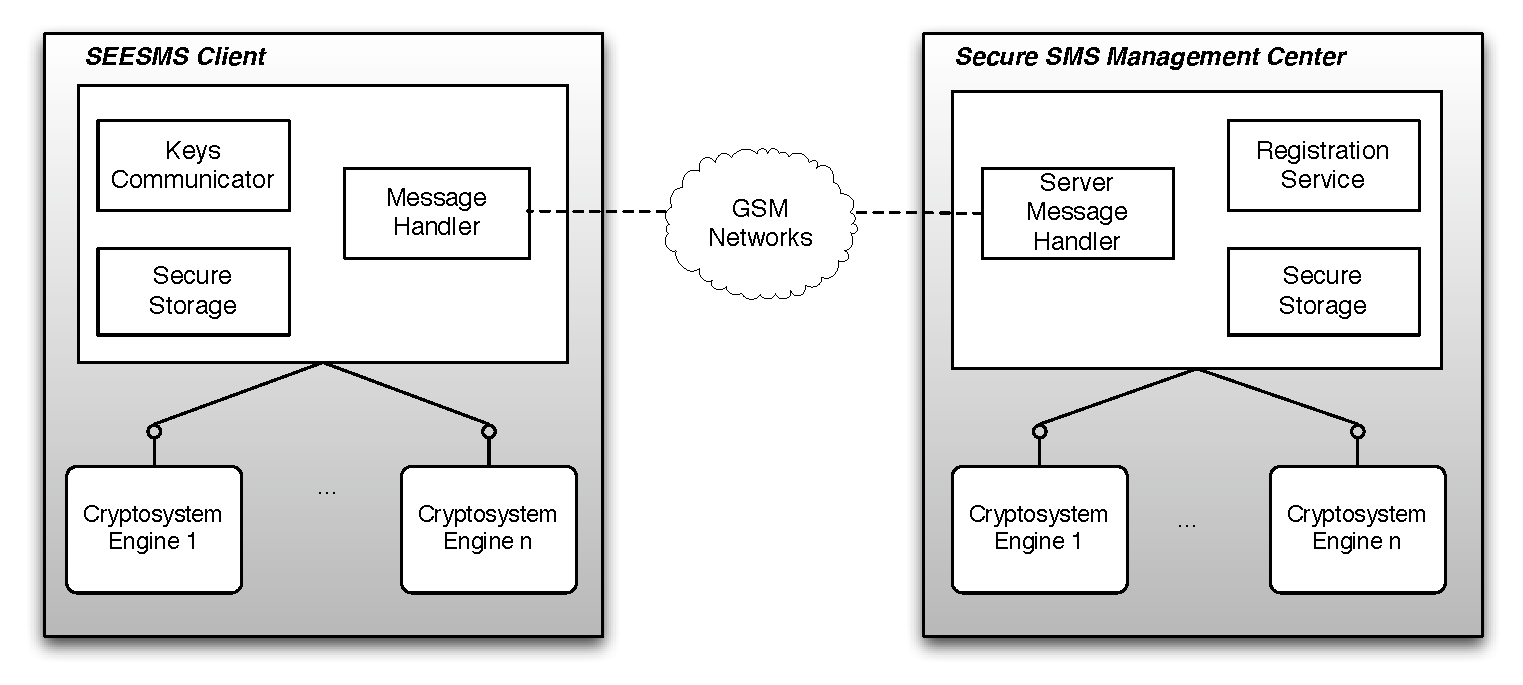
\includegraphics[width=9cm]{immagini/archJwhisper.eps}\\
  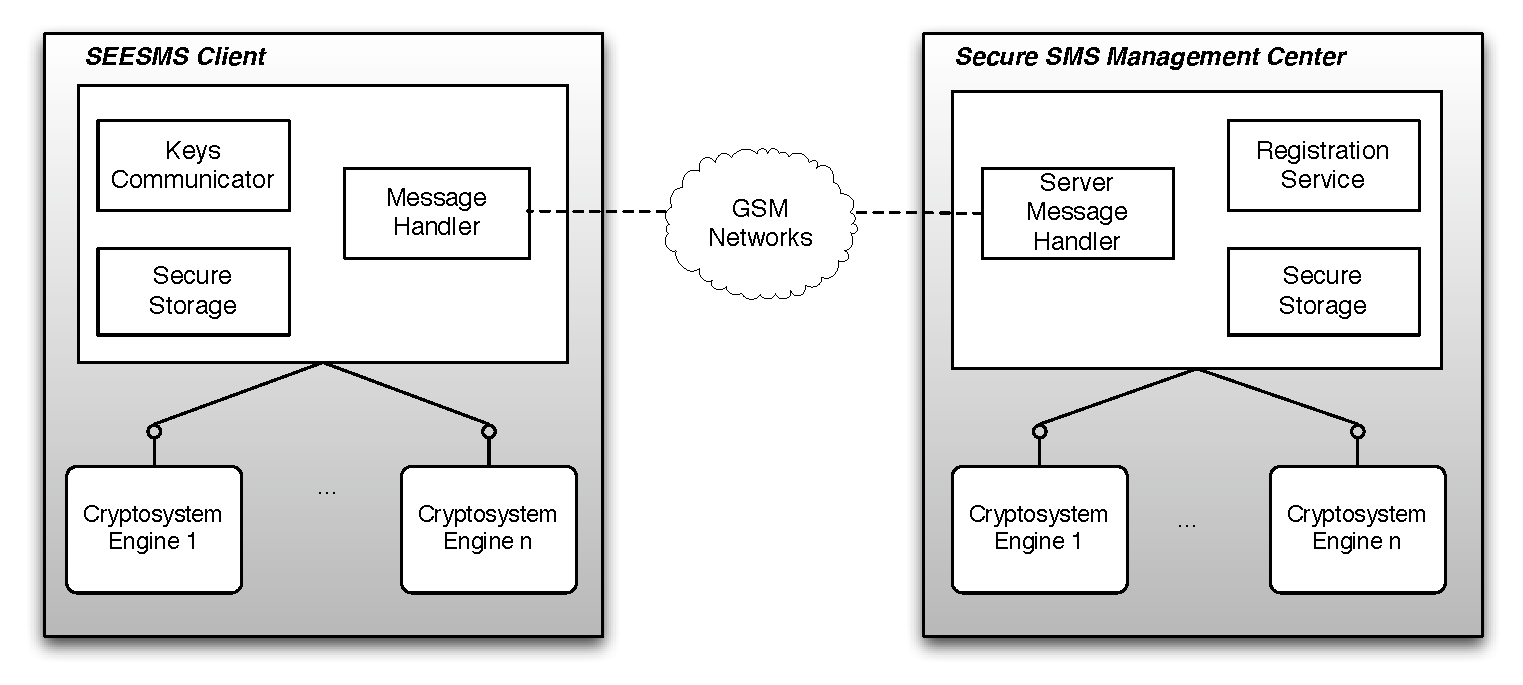
\includegraphics[width=12cm]{immagini/archJwhisper.pdf}\\
  \caption{The architecture of SEESMS}
  \label{fig:arch}
\end{center}
\end{figure}

We refer the interested reader to  \cite{DeSantis2010} for further information about the architecture and the inner workings of SEESMS.




%
%
%\section{The Architecture}
%The SEESMS framework adopts a hybrid architecture. If a user is interested in sending/receiving a secure message through SEESMS and has never used it before, then he has to contact a trusted third-party server, called Secure SMS Management Center (SSMC), to request a customized copy of the SEESMS client application. Similarly, if the user has already installed the SEESMS client, but does not own the public-key of the recipient of the message (or the public-key of the user who sent him a secure SMS message), he has to contact the SSMC server to ask for a copy of his key (this behavior is similar to the PGP key-servers). Instead, if the user already owns the public-key of his recipient, he will establish a direct communication in a peer-to-peer fashion, without further interaction with the SSMC server. Due to the use of a standard interface definition, all the cryptosystem engines have the same interface resulting in the ability to load them in the framework seamlessly.
%
%The following sections describe in details the SEESMS software components and their internal architecture, as described in Figure \ref{fig:arch}.
%
%
%
%
%\subsection{Secure SMS Management Center}
%The SSMC is in charge of handling the provisioning process, used to deliver to new users a customized copy of the SEESMS client application, and the key-distribution process, used to send the public-keys of registered users following a client request. The entire communication with clients is done by using signed SMS messages. The application includes the following modules:
%
%\begin{itemize}
%
%\item{\bf Registration Service (RS).} The RS is used to register new users, to provide them a copy of the SEESMS client application and to run key-exchange protocols with them. More details about these functions are provided in Sections \ref{subsec:provisioning} and \ref{subsec:keyexchange}.
%
%\item{\bf Server Message Handler (SMH).} The SMH is a module that can be used to exchange messages with another peer by means of SMS messages. It also includes the code needed to serialize/deserialize SMS messages and send/receive them through a GSM modem.
%
%% TODO: Includere reference ad AES
%\item{\bf Secure Storage (SS).} The SS implements a secure local storage area used to encrypt and to maintain sensitive data about the users that are registered to the service, such as their public-keys or their registration information. Data is encrypted using the AES symmetric cipher and stored in a relational database.
%
%% TODO: Includere references
%\item{\bf Cryptosystem Engines (CE).} The CE are the modules that take care of securing the messages exchanged with a remote user. Each CE carries the implementation of a cryptosystem and offers up to three standard set of functions: \textit{Key Generation}, \textit{Message Encryption/Decryption} and \textit{Message Signature/Verification}. These engines are used by the SSMC to implement the user registration phase and the key-exchange protocol. The current version of SEESMS includes the engines implementing ECC (ECDSA and ECIES), RSA and DSA.
%
%\end{itemize}
%
%\subsection{SEESMS Client}
%The SEESMS client application can be used by two parties to exchange encrypted and digitally signed SMS messages. It includes the following modules:
%
%\begin{itemize}
%
%\item{\bf Message Handler (MH).} The MH is responsible for sending and receiving secure SMS messages. It is a trimmed version of the SMH, not including the code needed to handle communication over a GSM modem.
%
%\item{\bf Secure Storage (SS).} The SS implements a secure local storage area used to hold sensitive data such as the cryptographic keys of a user.
%
%\item{\bf Cryptosystem Engines (CE).} Similarly to the SSMC case, the CE are used to implement the registration phase and the key-exchange protocol and, moreover, all the functions related to secure communications with another user.
%
%\item{\bf Keys Communicator (KC).} The KC module implements the client-side key-exchange protocol described in Section \ref{subsec:keyexchange} which is used to communicate to the SSMC the cryptographic keys generated by the client.
%\end{itemize}
%
%
%
%\section{SEESMS in Action}
%This section describes all the phases concerning the transmission of a secure message with SEESMS, assuming that the sender of the message has been using the framework for the first time.
%
%\subsection{Provisioning of the Client Application}
%\label{subsec:provisioning}
%A user interested in exchanging secure SMS messages using SEESMS firstly has to download and install a copy of the application using the RS offered by the SSMC.
%
%The provisioning process takes several steps:
%
%\begin{enumerate}
%\item The user registers on a web site hosted by the SSMC and asks for a copy of the client application.
%
%\item The RS generates a random string, called {\em nonce}, used in a subsequent phase of the registration process (step 4) to ensure that the user running the client application is the same that has requested for it. The nonce is split in two parts: the first part is communicated to the user through the registration web page and email, the second part is hard-coded in the copy of the client application that will be delivered to that user.
%
%\item The RS creates a software package containing the second part of the nonce generated in the previous step and the public-key of the server, and publishes it on a web site hosted by the SSMC. A WAP-Push message indicating the URL where the package (just created) has been published, is sent to the phone number specified by the user during the registration phase. The URL is randomly generated in order to avoid the possibility for an attacker to download a copy of the application instead of the legitimate user.
%
%\item The user downloads and installs the client on his mobile equipment and starts the application. During the first execution, the user inputs the part of the nonce received in step 2 of the registration process. The nonce is thus reassembled by combining this part with the other part embedded in the downloaded package in order to be used later (see the Section \ref{subsec:keyexchange}).
%\end{enumerate}
%
%At the end of the initialization, the user inputs a passphrase that is used to generate a pair of cryptographic keys which are subsequently stored in the SS of the client application.
%
%\subsection{Key-Exchange Protocol}
%\label{subsec:keyexchange}
%The public-keys generated by the user at the end of the provisioning phase must be sent to the SSMC server. The transmission must be performed in such a way to guarantee that the communication originates from the same user who downloaded the application in the previous phase.
%
%For the sake of simplicity, let us consider the case when the user has only one pair of cryptographic keys: the private-key ($\mathcal{SK}_{u}$) and the public-key ($\mathcal{PK}_{u}$). Moreover, let $\mathcal{N}_{u}$ be the part of the nonce generated and sent to the user during step 2 of the provisioning phase (see the Section \ref{subsec:provisioning}). The key-exchange protocol between a new user and the SSMC server requires the following steps.
%
%\medskip
%The client:
%\begin{enumerate}
%\item composes a message  $\mathcal{T}$  containing his phone number and a timestamp;
%\item computes $\mathcal{H}$ as the keyed-hash (HMAC) of $\mathcal{T}$$||$$\mathcal{PK}_{u}$ using the key $\mathcal{N}_{u}$;
%\item composes a message  $\mathcal{T'}$ containing $\mathcal{T}$ and $\mathcal{H}$;
%\item computes $\mathcal{D}$ as the result of the decryption of the message $\mathcal{T'}$ using the private-key $\mathcal{SK}_{u}$;
%\item sends to the server an SMS message $\mathcal{M}$ containing $\mathcal{D}$ and the public-key $\mathcal{PK}_{u}$.
%\end{enumerate}
%
%
%After receiving the message $\mathcal{M}$, the server:
%
%
%\begin{enumerate}
%\item reads from $\mathcal{M}$ the public-key $\mathcal{PK}_{u}$ and the value $\mathcal{D}$;
%\item computes $\mathcal{T'}$ as the result of the encryption of $\mathcal{D}$ with the public-key $\mathcal{PK}_{u}$ contained in $\mathcal{M}$;
%\item extract from $\mathcal{T'}$ the fields $\mathcal{T}$ and $\mathcal{H}$;
%\item computes $\mathcal{H'}$ as the keyed-hash (HMAC) of $\mathcal{T}$$||$$\mathcal{PK}_{u}$ using, as a key, the nonce $\mathcal{N}_{u}$ generated for that user;
%\item extracts from $\mathcal{T}$ the phone number of the user, the timestamp and keyed-hash $\mathcal{H}$;
%\item checks the timestamp to avoid reply attack. If the check is successful, compares the extracted tag $\mathcal{H}$ with $\mathcal{H'}$ computed at step $4$. If the tags are identical, the public-key of the user is saved in the SS, a signed confirmation SMS is sent to the client and the registration process ends correctly. Otherwise, the registration process ends with a failure.
%\end{enumerate}
%
%From this moment on, all the SMS messages involved in the communications between the client and the SSMC will be signed. Moreover, due to the HMAC verification, Man-In-The-Middle attacks will be easily detected and reported.
%
%
%\subsection{Exchange of a Secure Message}
%SEESMS implements secure SMS messages exchange by using binary SMS messages rather than traditional textual messages. Each binary SMS message can hold $140$ bytes (equivalent to the $160$ 7-bit characters used for textual messages). The $140$ bytes are partitioned as shown in Figure \ref{fig:SMSPayload}.
%
%\begin{figure}[ht]
%\begin{center}
%%%%  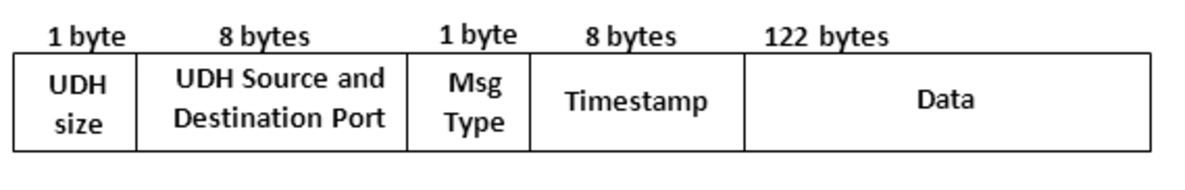
\includegraphics[width=9cm]{immagini/SMSPayload.eps}\\
%  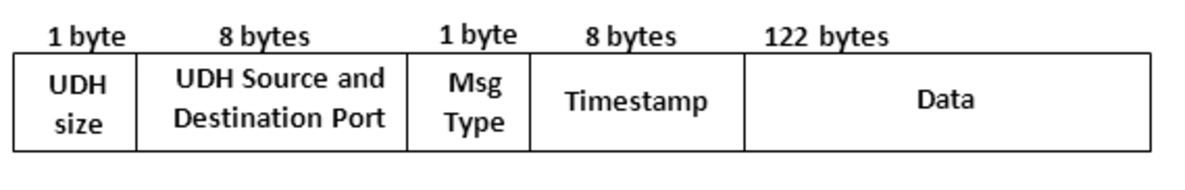
\includegraphics[width=12cm]{immagini/SMSPayload.pdf}\\
%  \caption{SMS Payload organization}
%  \label{fig:SMSPayload}
%  \end{center}
%\end{figure}
%
%The first two fields (i.e., \emph{UDH size} and \emph{UDH Source and Destination Port}) represent the SMS User Data Header (UDH), a standard extension to the GSM specifications which allows to deliver the message to an application listening on a specific port at the receiver ME. The subsequent $9$ bytes are used to specify the message type ($1$ byte) and the timestamp ($8$ bytes). The \emph{Msg Type} field indicates the cipher used to process the current message and the key length used by the cipher (e.g., 1024 bits RSA public-key or 160 bits ECIES encrypted text). The \emph{Timestamp} field marks the time when the message has been sent. Finally, the \emph{Data} field is used by the chosen cryptosystem to carry the content of the message together with cryptographic tokens such as signatures, public-keys and so on. 
%
%Suppose a registered user is interested in sending a secure SMS message to another user through SEESMS. If he already owns the public-key of the recipient, then he has just to input which cryptosystem to use, the corresponding security parameters and the text of the message to be sent. The input message is processed by the chosen cryptosystem and one or more SMS messages are generated and sent to the recipient. If the public-key of the recipient is not known, then the user application sends to the SSMC server the phone number of the recipient, asking for his public-key. The SSMC responds with an SMS signed with his own private-key, containing a copy of the public-key of the recipient (if it exists).
%
%% As examples, the Figures \ref{fig:ECIESPayload} and
%% \ref{fig:ECDSAPayload} show the SMS payload for a message encrypted
%% with the ECIES cipher and for a message signed with the ECDSA signer
%% using 192 bits keys respectively. It can be noticed in Figures
%% \ref{fig:ECIESPayload} and \ref{fig:ECDSAPayload}, using elliptic
%% courve cryptography with 192-bit keys (equivalent to 1536 bit RSA
%% keys, see \ref{table:secLevels}), in the \emph{Data} about 50 bytes
%% remain available for the user message. The \emph{Data} field size is
%% not a problem the GSM standards define SMS concatenation. The majority
%% of mobile operators allow to concatenate up to 4 SMS and thus
%% obtaining $140+140+140+121=541$ bytes at maximum for the data field.
%
%% \begin{figure}[ht]
%%   \includegraphics[width=9cm]{immagini/ECIES192Payload.eps}\\
%%   \caption{SMS carrying 192 bits ECIES encrypted text}
%%   \label{fig:ECIESPayload}
%% \end{figure}
%
%% \begin{figure}[ht]
%%   \includegraphics[width=9cm]{immagini/ECDSA192Payload.eps}\\
%%   \caption{SMS carrying 192 bits ECDSA signed text}
%%   \label{fig:ECDSAPayload}
%% \end{figure}
%


\section{Experimental Setup}
\label{sec:exp}
Several tests have been conducted in order to evaluate the efficiency of the cryptographic algorithms available with SEESMS and to determine which security configuration would better suit the needs of a user. The framework is designed to handle any kind of cryptographic operations. Nevertheless, in the tests have been evaluated only the signature operations because otherwise it would have implied a longer exposition. Moreover, this choice is justified by the observation that signing operations have a computational complexity similar to the encryption ones.

This section briefly discusses the cryptosystems involved in our experiments and describes the security equivalence with respect to their key sizes.



\section{Previous Experimental Results}
\label{sec:experimental results}

The original description of SEESMS was accompanied by the results of a preliminary set of experiments. These experiments were aimed at assessing the performance of the cryptosystems supported by SEESMS, when used to secure communication among different types of mobile devices, using different combinations of security parameters. All the measurements were conducted on two widely available mobile devices: the Nokia N95-8GB (Symbian OS 9.2 - CPU 332 MHz) and the HTC S620 (Windows Mobile 5.0 - CPU 201 MHz). Each test was repeated 200 times and the resulting data averaged. Several performance metrics were collected, most of them were related to the time needed to accomplish cryptographic operations.

The cryptosystems included in the original experimentations were RSA, DSA and ECDSA. The RSA cryptosystem is the most widely used public-key based cryptosystem. It may be used to provide both secrecy and digital signatures and its security is based on the intractability of the Integer Factorization Problem (IFP). The Digital Signature Algorithm (DSA) is the first digital signature scheme to be recognized by a government. Its security relies on the Discrete Logarithm Problem (DLP) that is shown to be as hard as the IFP. The Elliptic Curve Digital Signature Algorithm (ECDSA) has been proposed as an ANSI X9.62 standard. Unlike the Discrete Logarithm Problem (DLP) and the Integer Factorization Problem (IFP), the Elliptic Curve Discrete Logarithm Problem (ECDLP) has no subexponential-time algorithm. For this reason, the ``strength-per-key-bit'' is substantially greater in an algorithm that uses elliptic curves.
A detailed presentation of the security-equivalent configurations is described in \citet{sec2} and summarized in Table \ref{table:secLevels}.

\begin{table}[ht]
\caption{Rough Comparison of RSA and ECDSA Key Size Security Levels
  (in bits)}
\centering % used for centering table
\begin{tabular}{|c|c|} % centered columns (4 columns)
\hline\hline %inserts double horizontal lines
ECDSA & RSA \\ [0.5ex] % inserts table
%heading
\hline\hline % inserts single horizontal line
112 & 512  \\ % inserting body of the table
128 & 704  \\
160 & 1.024 \\
192 & 1.536 \\
224 & 2.048 \\
256 & 3.072 \\ [1ex] % [1ex] adds vertical space
\hline %inserts single line
\end{tabular}
\label{table:secLevels} % is used to refer this table in the text
\end{table}


Most of the observed results were in line with the theoretical expectations, however there were some noteworthy exceptions. This was the case of the experiments concerning the generation of signatures using, respectively, the ECDSA and the RSA cryptosystems. Despite the common expectations, ECDSA performed very poorly  and revealed to be often slower than RSA, even when using long keys. Such a behavior is likely to be due to some issues in the design and/or the implementation of the ECDSA cryptosystem coming with the Bouncy Castle library. In the rest of this section, we briefly summarize the outcoming of those tests, mainly focusing on the results which required a further investigation.




%The tests compare the performance of RSA, DSA and ECDSA when signing random messages of fixed length using an increasing level of security. A message is signed by hashing it using the SHA1 algorithm and, then, signing the resulting text using one of the supported algorithm. All the cryptographic algorithms have been evaluated using different key sizes ranging from $512$ to $3.072$ bits, for RSA and DSA algorithms, and from $112$ to $256$ bits, for ECDSA. This work analyzes the performance of the three algorithms by comparing them using the security-equivalent configurations described in Table \ref{table:secLevels}. For the sake of brevity, in the results have been reported only RSA and DSA security configurations, thus referring the interested reader to the above mentioned table for the equivalent ECDSA security configuration.
%




\subsection{Time Efficiency}
The test evaluated the time efficiency of the supported cryptosystems by measuring separately the time elapsed to sign and to verify a single generic message. These two measurements report the time that the user has to wait every time he sends and receives a secure SMS message on the ME, provided that it has already been configured. The execution times was evaluated by using the {\tt System.currentTimeMillis()} primitive available within the J2ME framework.

% Third, we consider the memory usage during the
% transmission of a secure SMS. Fourth, we energy consumption related to
% the transmission of a secure SMS.

% The memory usage has been
% determined by running our framework in the standard Sun Java Wireless
% Toolkit(WTK) device emulator\footnote{The Sun Java Wireless Toolkit is
%   a toolbox for developing wireless applications that are based on
%   J2ME's Connected Limited Device Configuration (CLDC) and Mobile
%   Information Device Profile (MIDP). The toolkit includes the
%   emulation environments, performance optimization and tuning
%   features, documentation, and examples.} since there were no memory
% profiling instructions available with mobile devices. Finally, the
% energetic consumption has been measured using the Nokia Energy
% Profiler \citep{NEP} with the N95 development kit.

% To test the algorithm on mobile phones we implemented a minimal midlet
% for each algorithm. The midlet consist of a simple form object used to
% print the test results and a minimal menu to start the test. The
% cryptographic primitives were provided by the Bouncy Castle J2ME
% library. We used the bytecode obfuscator Pro Guard which is able to
% remove unused class and package from the midlet JAR and hence
% noticeably reducing the JAR size. The energy consumption test have
% been done on the N95-8GB using a fully charged battery

% \subsection{Signature generation}



Figure \ref{fig:HTCSign} and \ref{fig:N95Sign} show the time needed to digitally sign an SMS using, respectively, an HTC S620 and a Nokia N95-8GB. Despite the expectations, the RSA algorithm performs generally better than ECDSA. The DSA algorithm is slightly faster than RSA for small key sizes, however it is only available with keys no longer than $1.024$ bits. The only case where ECDSA outperforms RSA is when using very long keys (near $3.072$ bits). This behavior is worth of further investigation because it is widely known from literature that ECDSA should perform generally faster than RSA and DSA.

\begin{figure}[ht]
\begin{center}
%%%  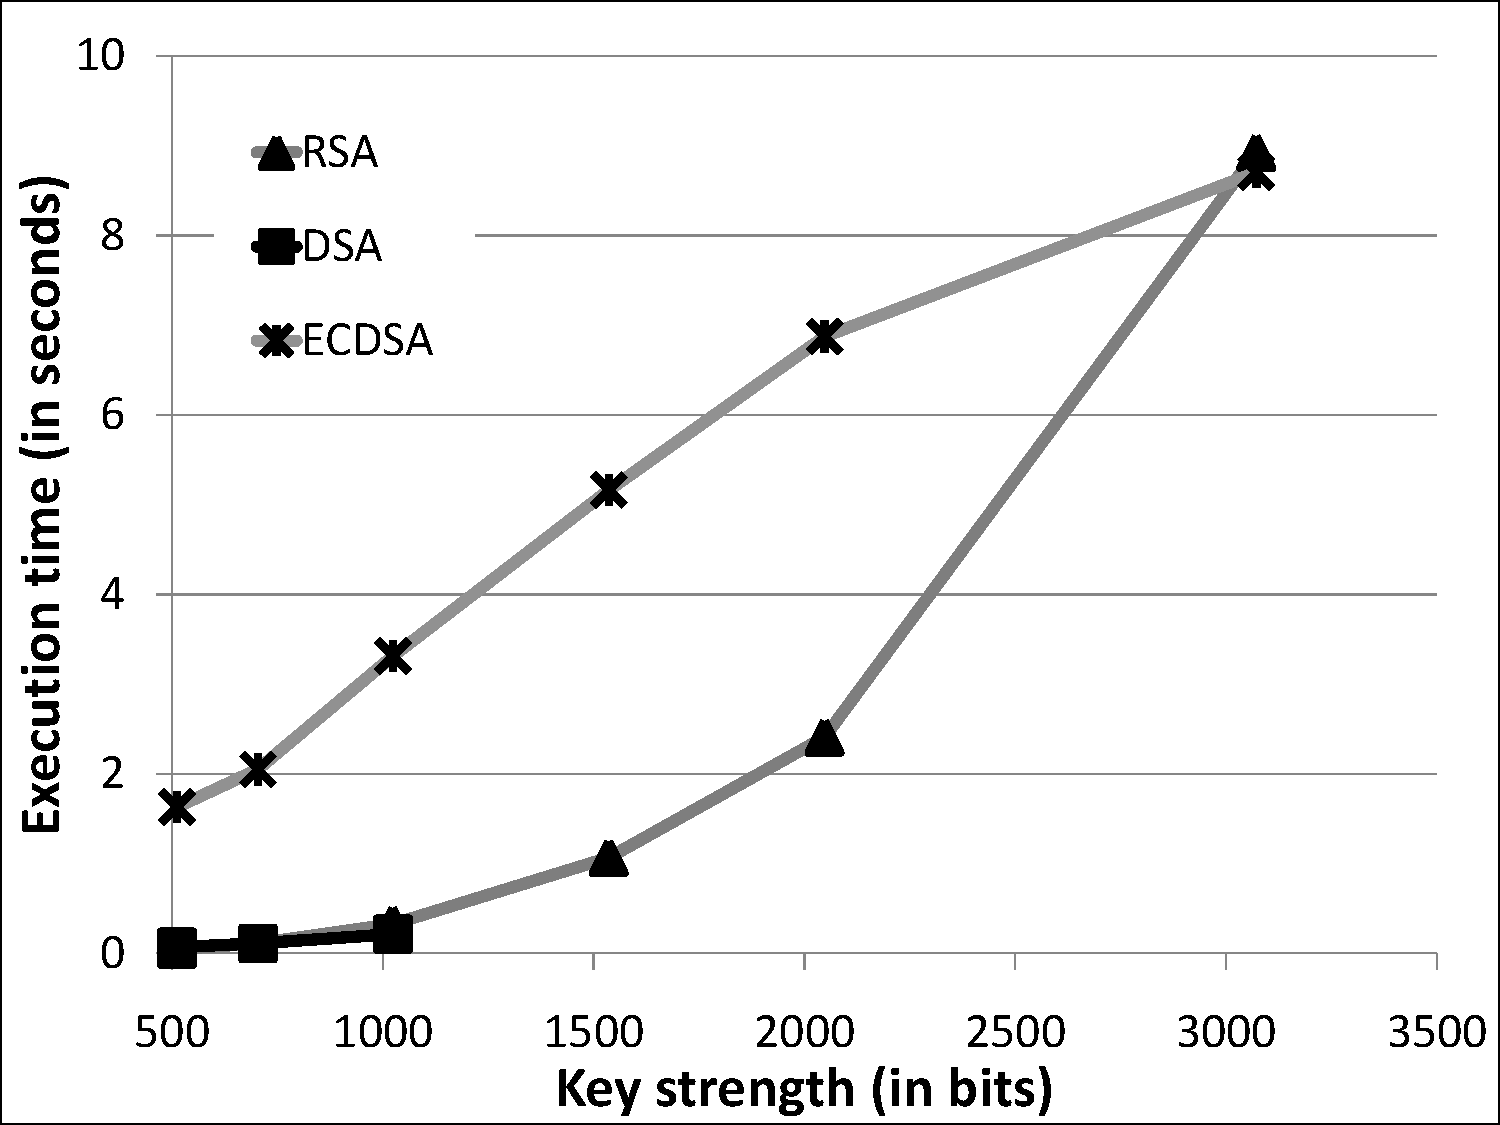
\includegraphics[width=9cm]{immagini/HTCSign.eps}\\
  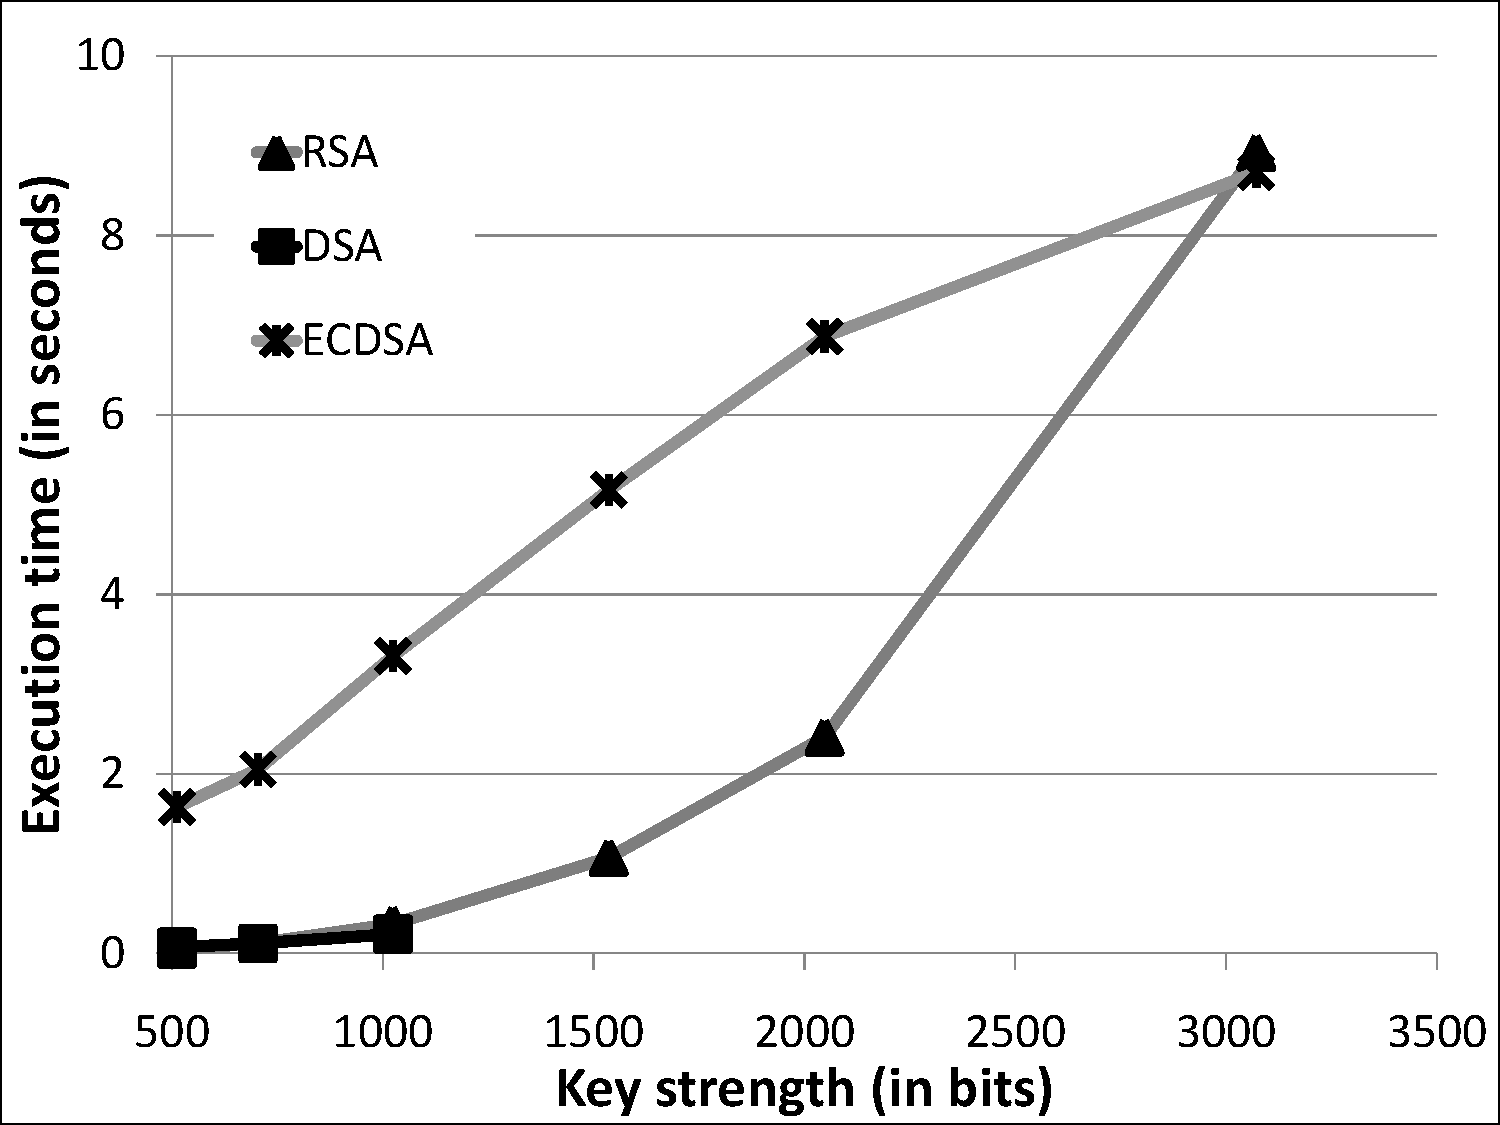
\includegraphics[width=7cm]{immagini/HTCSign.pdf}\\
  \caption{HTC S620 average signature generation time}
  \label{fig:HTCSign}
\end{center}
\end{figure}

\begin{figure}[ht]
\begin{center}
%%%  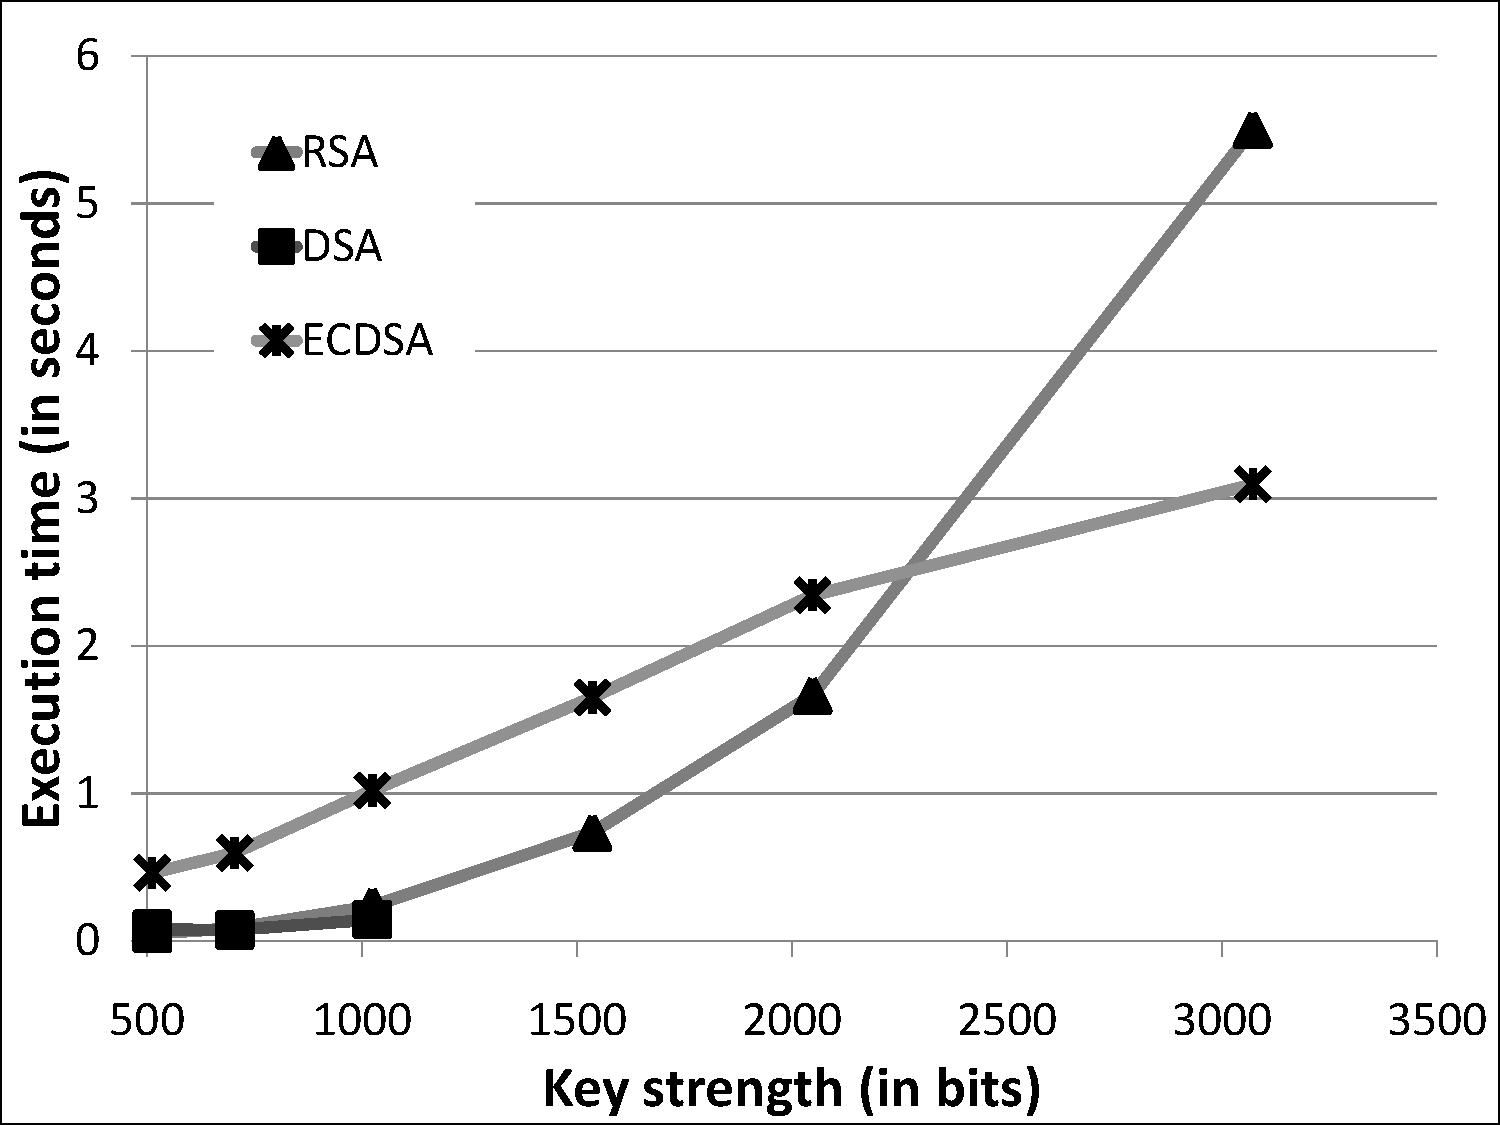
\includegraphics[width=9cm]{immagini/N95Sign.eps}\\
  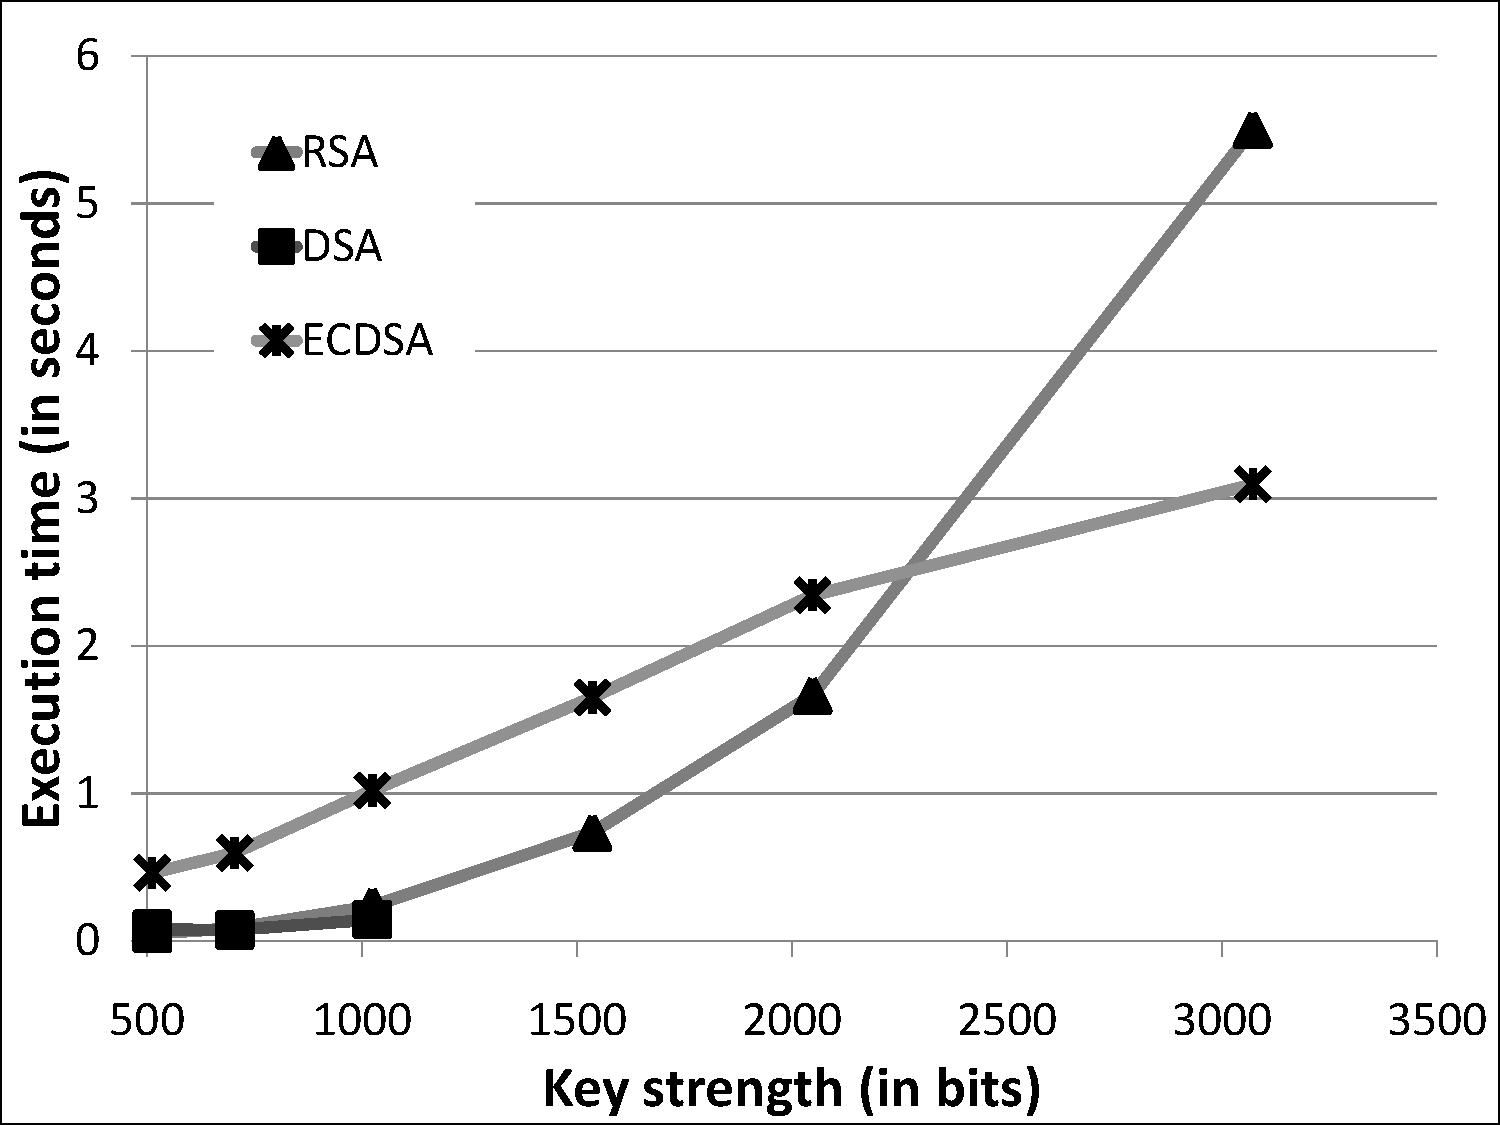
\includegraphics[width=7cm]{immagini/N95Sign.pdf}\\
  \caption{Nokia N95-8GB average signature generation time}
  \label{fig:N95Sign}
\end{center}
\end{figure}
% An important performance measure to consider is the time need by the first execution of the signing algorithm as soon as the midlet starts. In the Table \ref{table:N95FirstSign} we report the tim spent for the first signing operation on N95-8GB.

% \begin{table}[ht]
% \caption{N95-8GB first signing operation}
% \centering % used for centering table
% \begin{tabular}{c|c c c} % centered columns (4 columns)
% \hline\hline %inserts double horizontal lines
% Key strength (bit) & RSA (ms) & DSA (ms)& ECDSA(ms) \\ [0.5ex] % inserts table
% %heading
% \hline\hline % inserts single horizontal line
% 512  & 395   & 94  & 567  \\ % inserting body of the table
% 704  & 440  & 177 & 900  \\
% 1024 & 666  & 280 & 1458 \\
% 1536 & 1245 & -   & 2282 \\
% 2048 & 1735 & -   & 2396 \\
% 3072 & 5562 & -   & 3611 \\ [1ex] % [1ex] adds vertical space
% \hline %inserts single line
% \end{tabular}
% \label{table:N95FirstSign} % is used to refer this table in the text
% \end{table}

% As we can see from Table \ref{table:N95FirstSign} the time needed for the first execution of the signing algorithm is considerably slower than the medium value reported in Figure \ref{fig:N95Sign}. From our approach we will consider this table in order to evaluate the time needed for a secure message exchange.

% \subsection{Signature verification}

Concerning the signature verification process, the RSA algorithm performs much better than ECDSA and slightly better than DSA (see Figures \ref{fig:HTCVerify} and \ref{fig:N95Verify}). This is partially what it is expected because, for public-key operations, RSA can benefit of the public exponent size which, according to the algorithm, is often a prime close to a power of 2 (e.g., $3$, $5$, $7$, $17$, $257$, $65.537$). However, we were surprised to notice such a big difference between the performance of RSA and ECDSA. For example, when using key sizes of $1.024$ bits, RSA ($\sim15$ ms) was approximately $300$ times faster than ECDSA ($\sim4500$ ms) on a HTC S620 phone.

\begin{figure}[ht]
\begin{center}
%%%  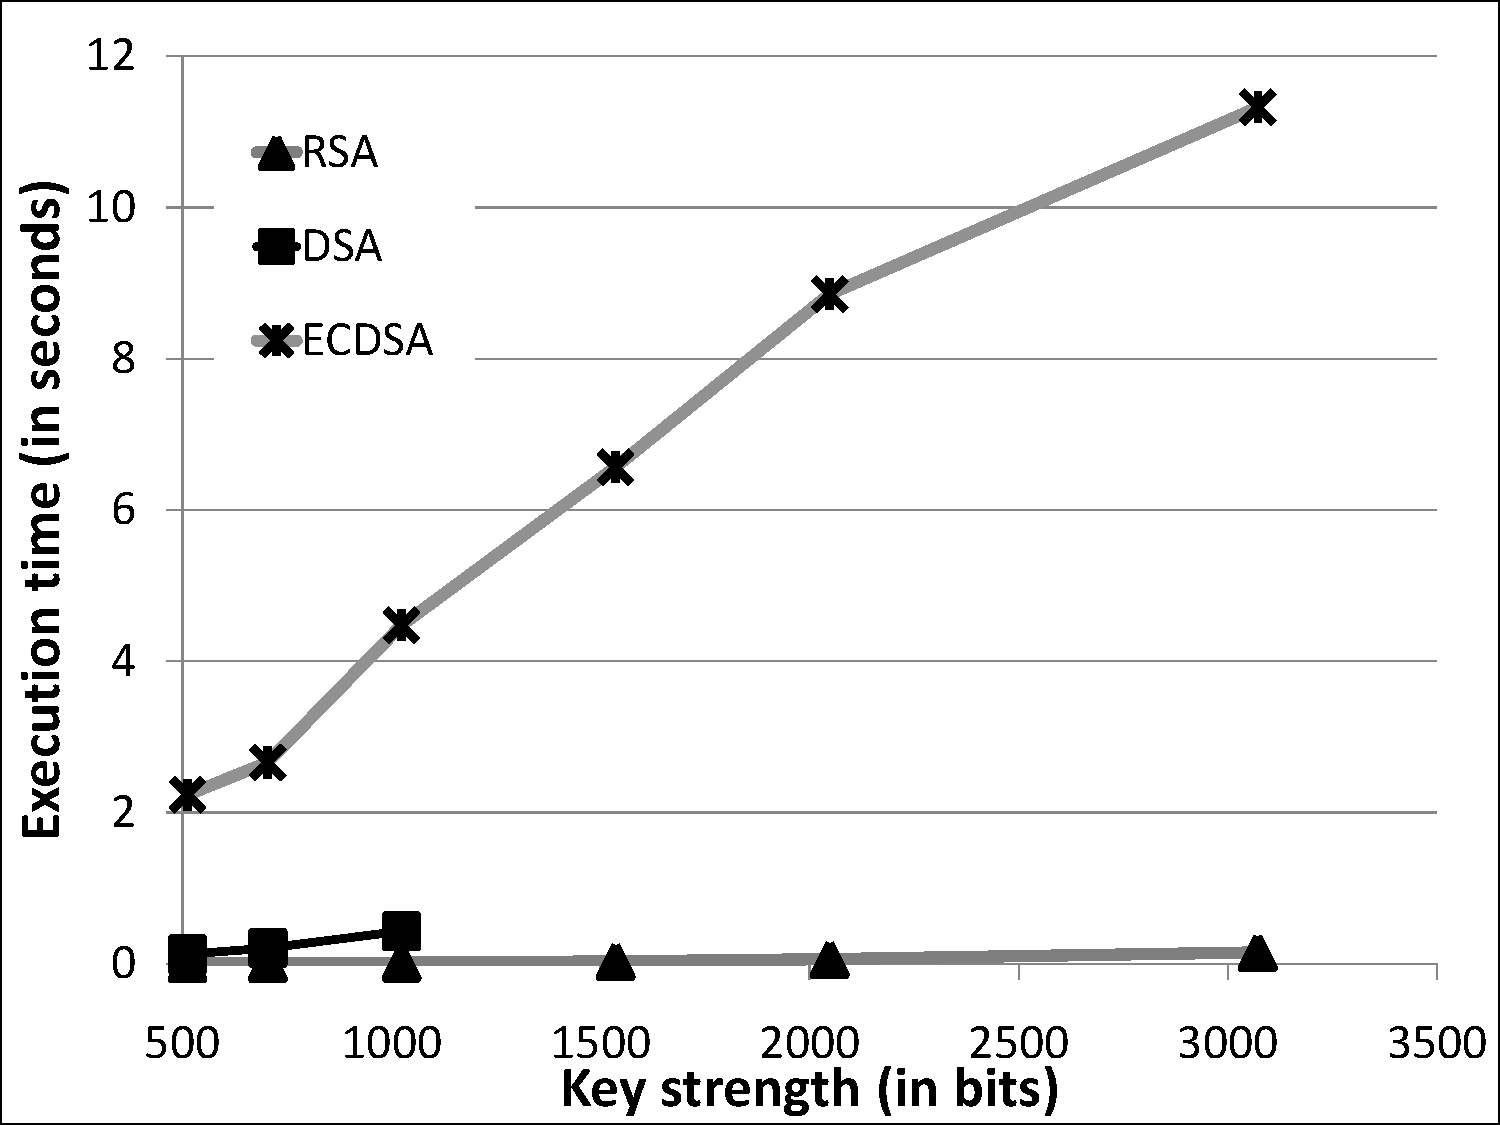
\includegraphics[width=9cm]{immagini/HTCVerify.eps}\\
  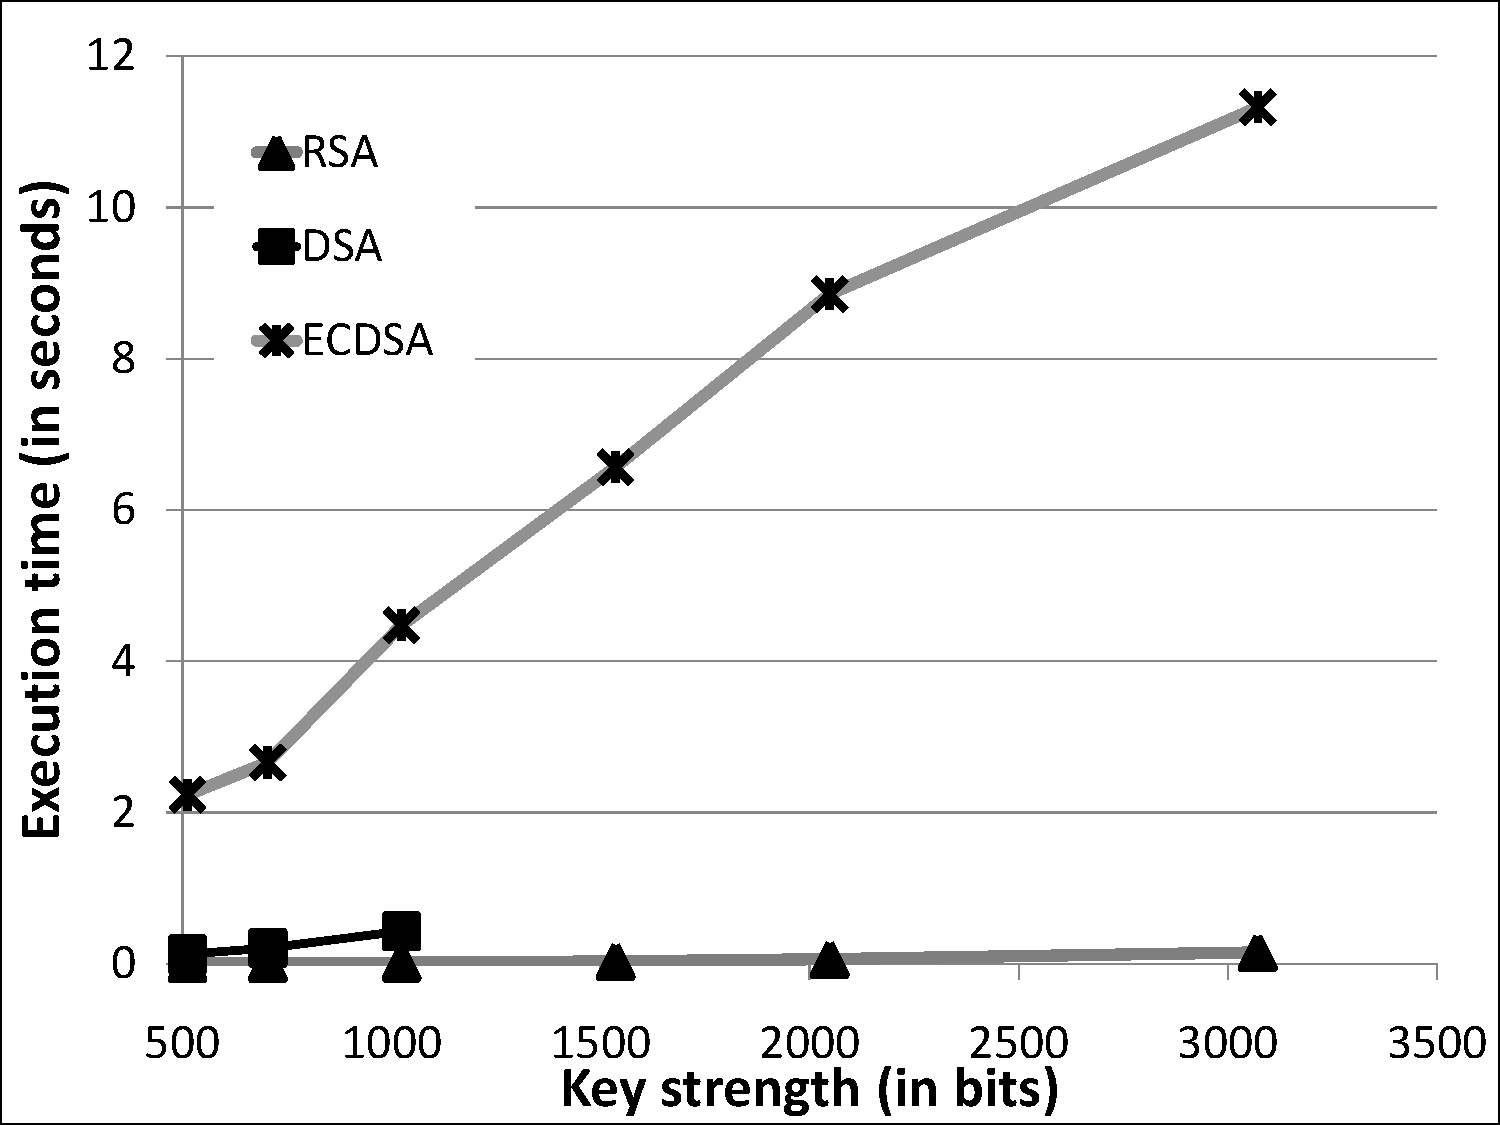
\includegraphics[width=7cm]{immagini/HTCVerify.pdf}\\
  \caption{HTC S620 average signature verification time}
  \label{fig:HTCVerify}
\end{center}
\end{figure}

\begin{figure}[ht]
\begin{center}
%%%  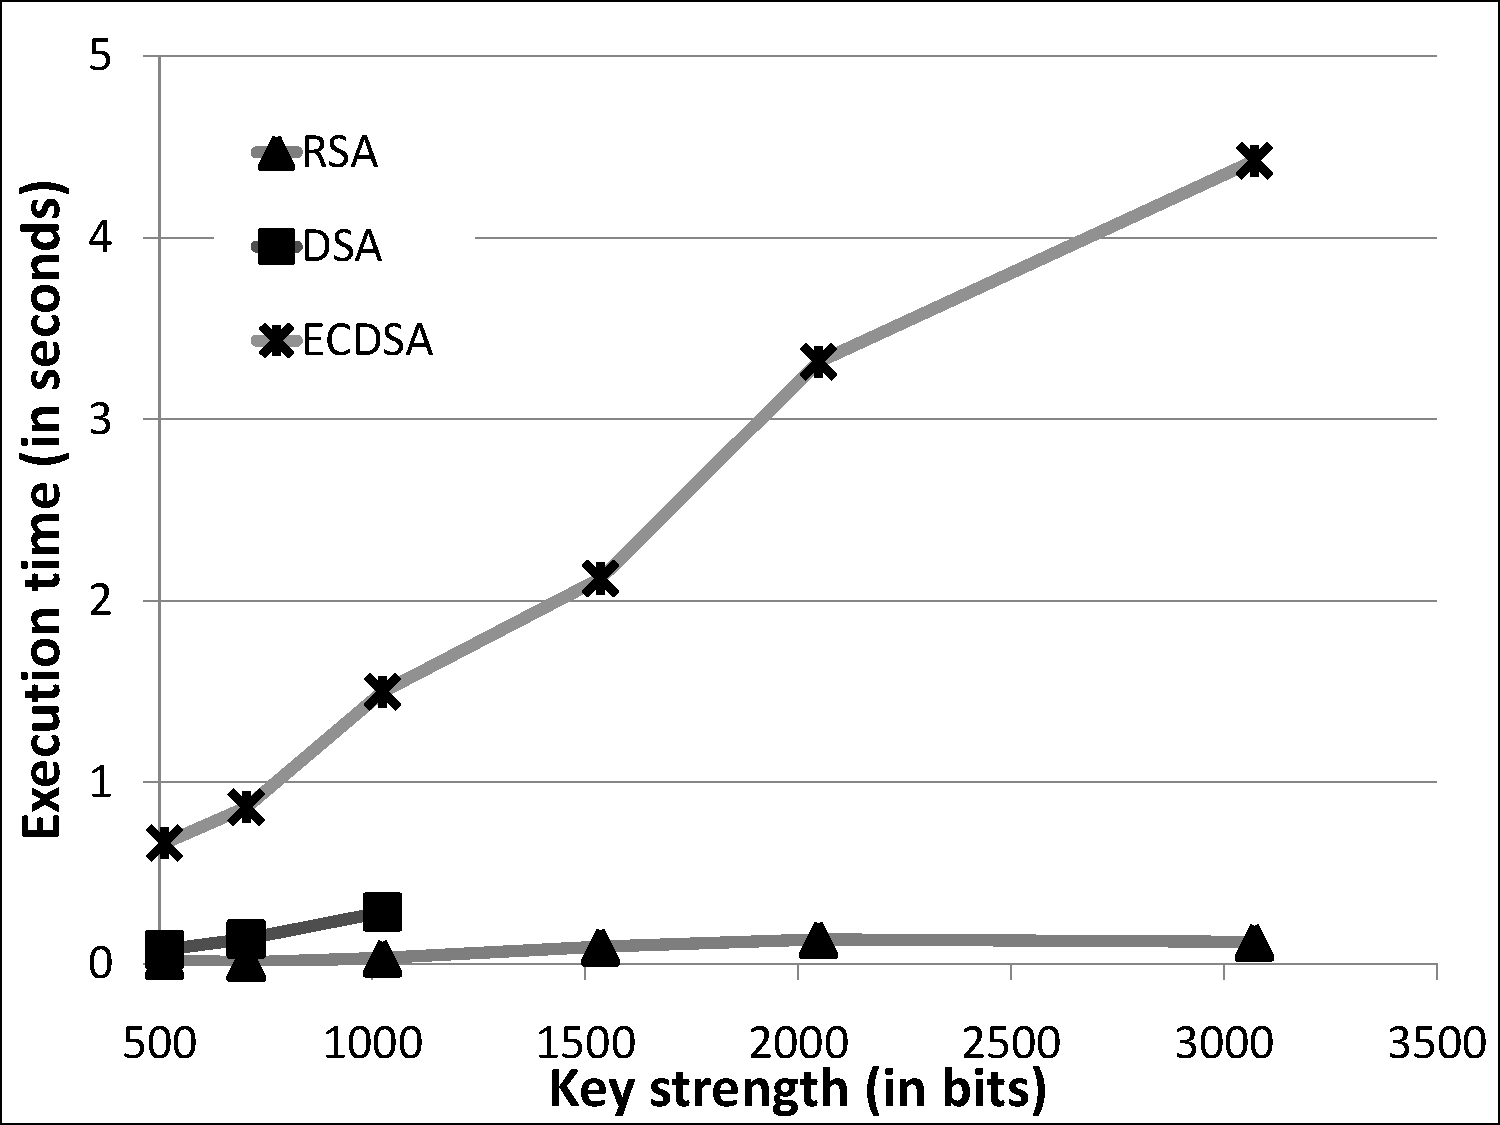
\includegraphics[width=9cm]{immagini/N95Verify.eps}\\
  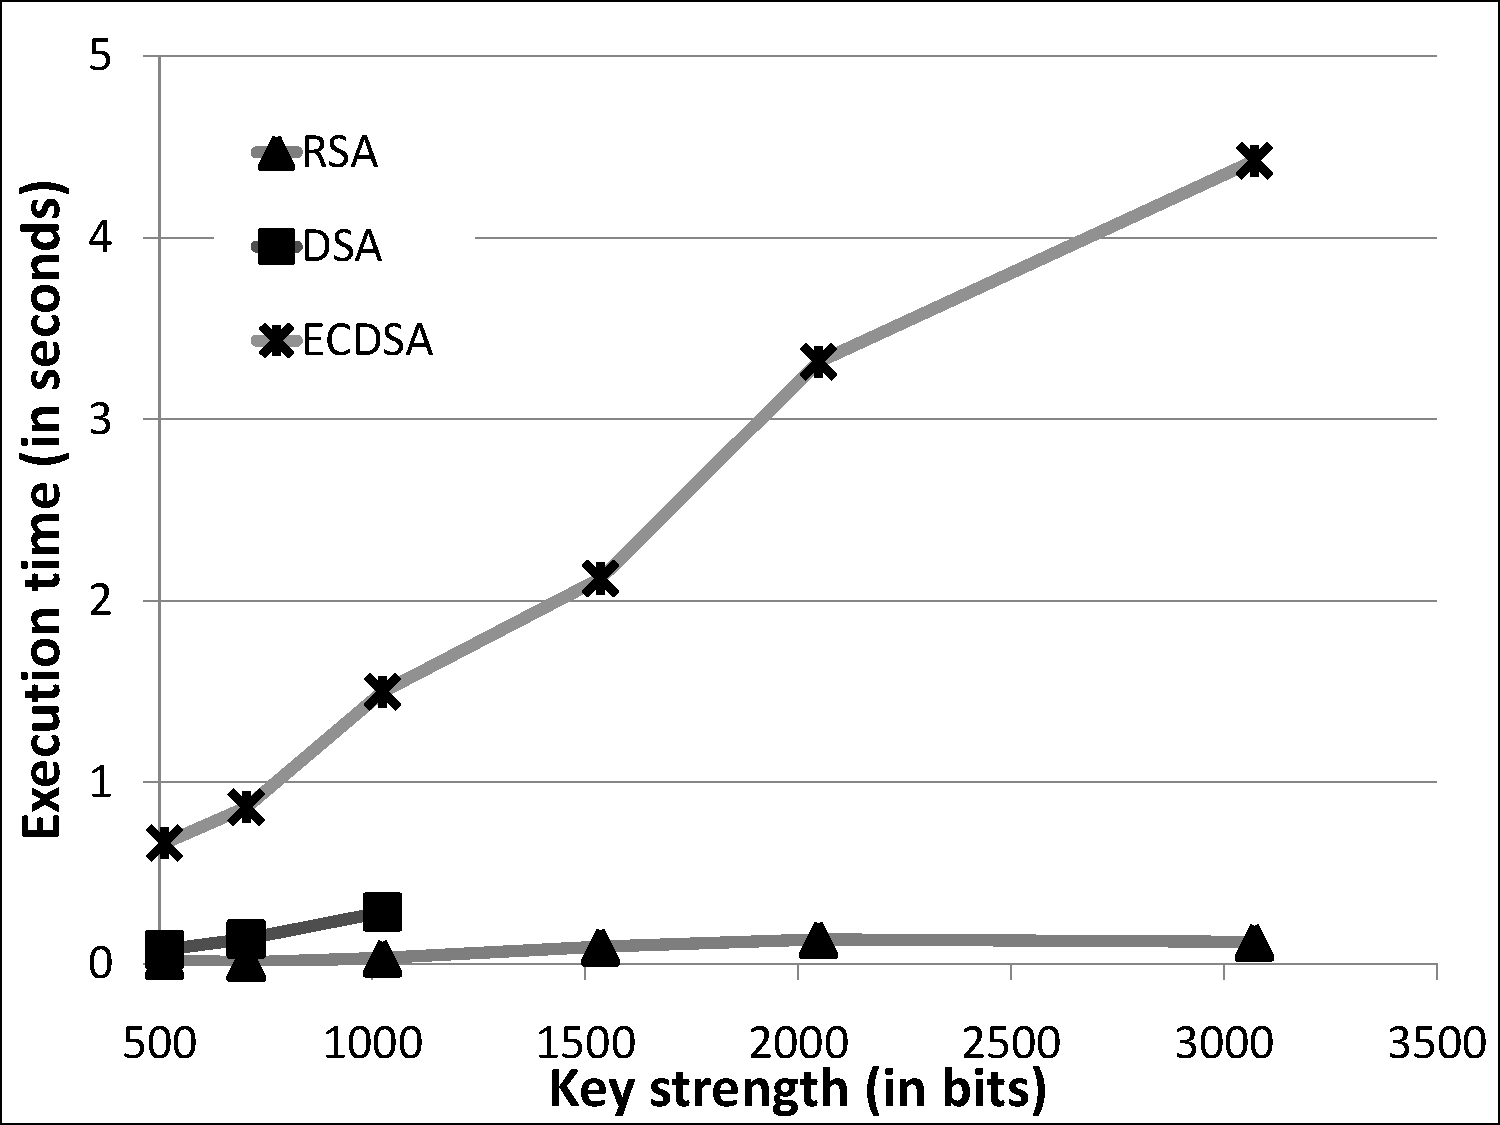
\includegraphics[width=7cm]{immagini/N95Verify.pdf}\\
  \caption{N95-GB average signature verification time}
  \label{fig:N95Verify}
\end{center}
\end{figure}

These results seem to indicate that ECDSA performs, in practice, worst than expected. In order to further investigate this behavior, the memory usage was profiled when signing a message by mean of the Sun Java Wireless Toolkit Memory Profiler (WTK). The results, presented in Figures \ref{fig:MemoryRSA}, \ref{fig:MemoryDSA} and \ref{fig:MemoryECDSA}, show that not only ECDSA has much higher memory requirements than RSA and DSA, but also that during the lifespan of a signature generation, a significant amount of memory is apparently and repeatedly allocated and deallocated. This behavior is likely to be due to the activity of the Garbage Collector module used by the Java virtual machine which runs the application. This module is automatically activated by the system whenever the memory usage of an application reaches a certain upper threshold, and its reaction is to reclaim (and to free) all the memory that is not in use anymore. The overhead due to memory allocations and deallocations is likely to be responsible for the bad performance of ECDSA. As shown below, even the bigger power consumption with the respect to the other two cryptosystems is likely to depend from this reason. The other two cryptosystems, instead, show simpler memory profiles. In their case, since the maximum amount of memory threshold is never reached, the use of the Java Garbage Collector module is reduced. In Figures \ref{fig:MemoryRSA}, \ref{fig:MemoryDSA} and \ref{fig:MemoryECDSA} the horizontal scale axis is not relevant because it depends on the average user-input time.

\begin{figure}[ht]
\begin{center}
%%%  \includegraphics[width=9cm]{immagini/Memory.eps}\\
  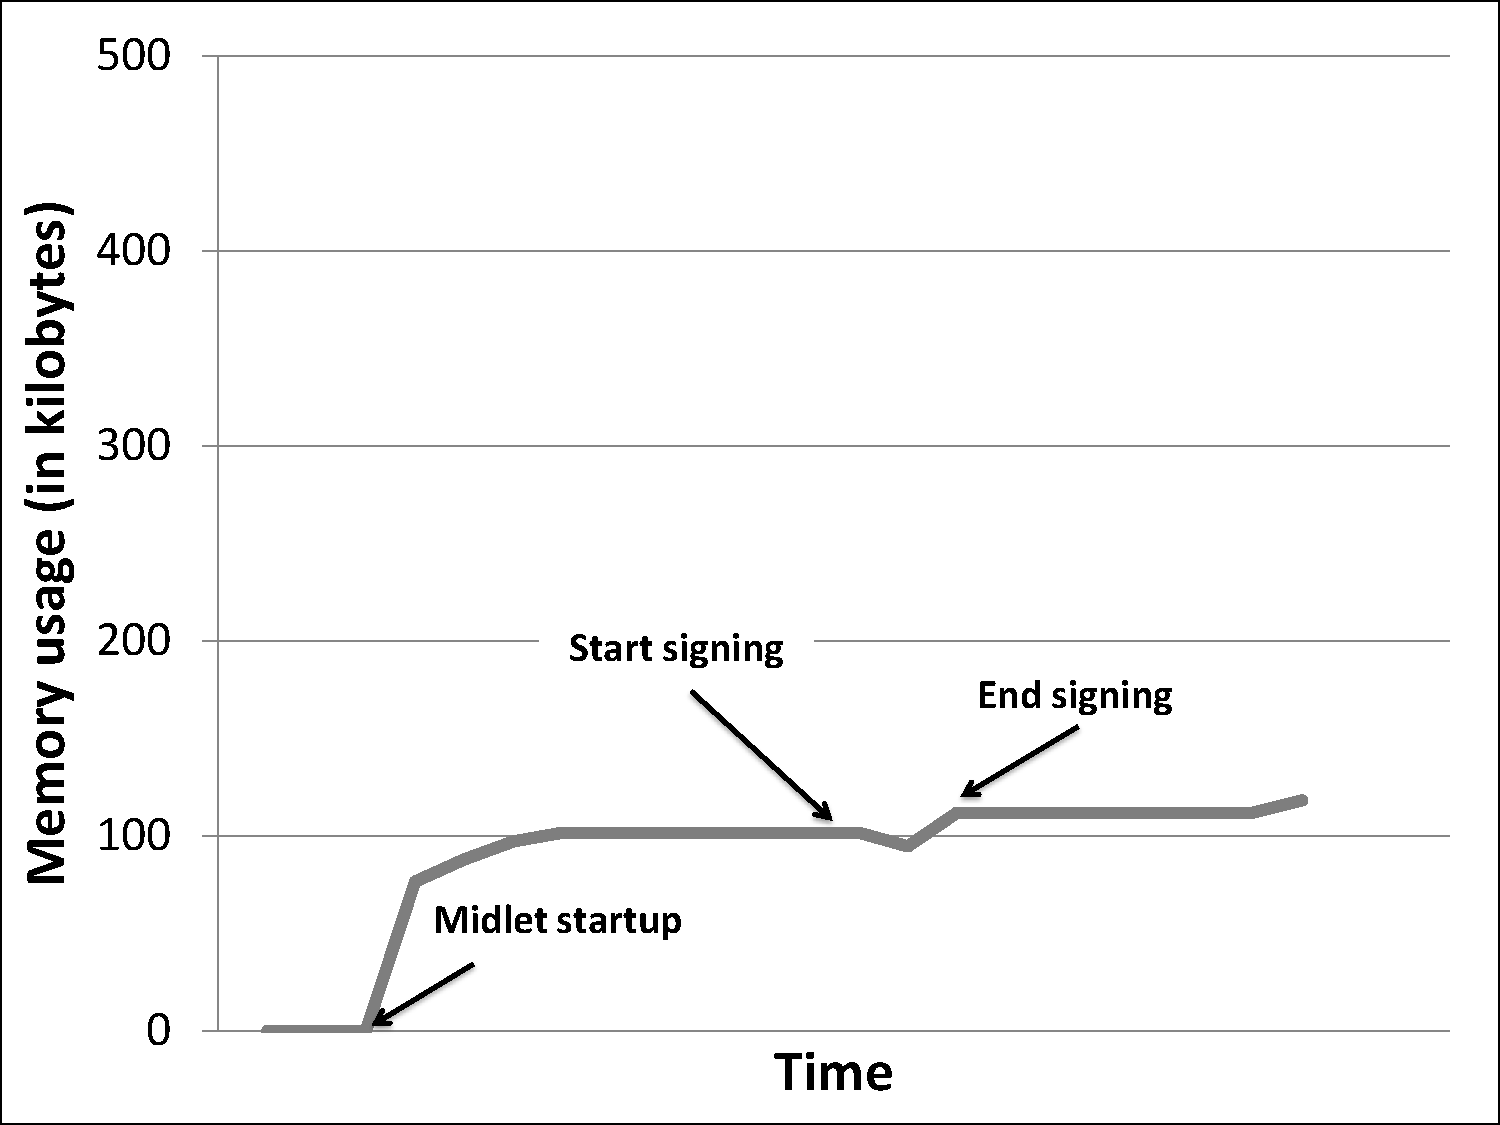
\includegraphics[width=7cm]{immagini/MemoryRSA.pdf}\\
  \caption{Memory usage profile of \textbf{RSA} when processing a 1024-bit signature}
  \label{fig:MemoryRSA}
\end{center}
\end{figure}

\begin{figure}[ht]
\begin{center}
%%%  \includegraphics[width=9cm]{immagini/Memory.eps}\\
  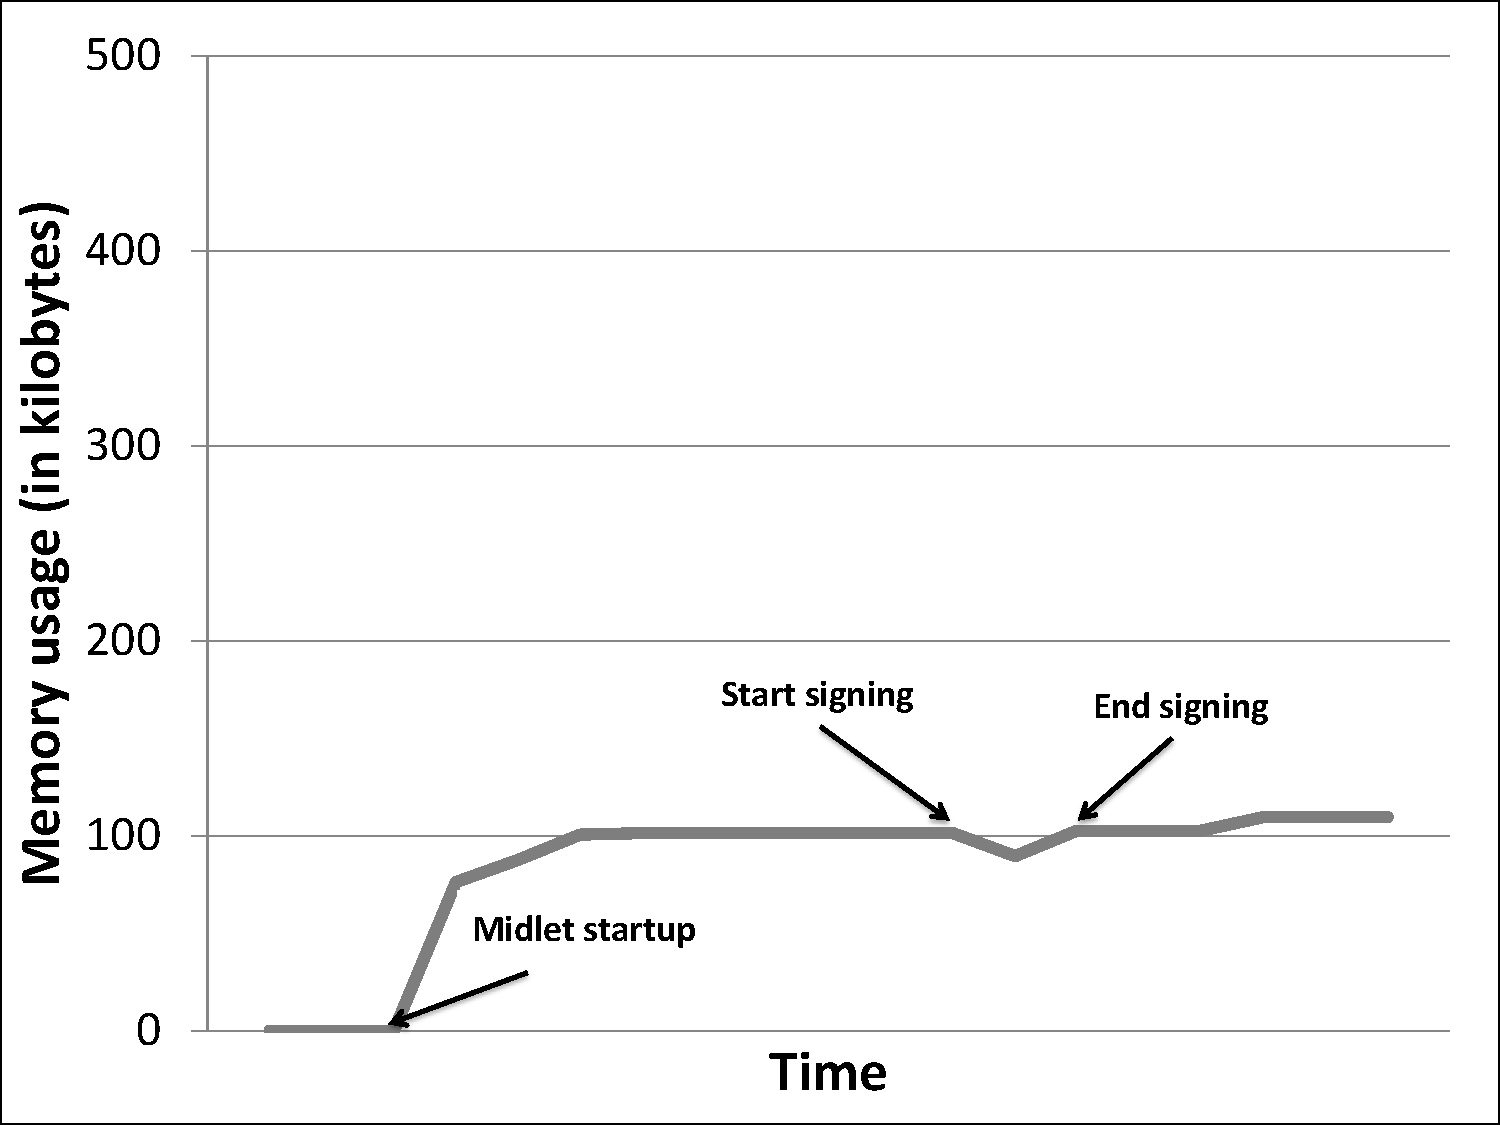
\includegraphics[width=7cm]{immagini/MemoryDSA.pdf}\\
  \caption{Memory usage profile of \textbf{DSA} when processing a 1024-bit signature}
  \label{fig:MemoryDSA}
\end{center}
\end{figure}

\begin{figure}[ht]
\begin{center}
%%%  \includegraphics[width=9cm]{immagini/Memory.eps}\\
  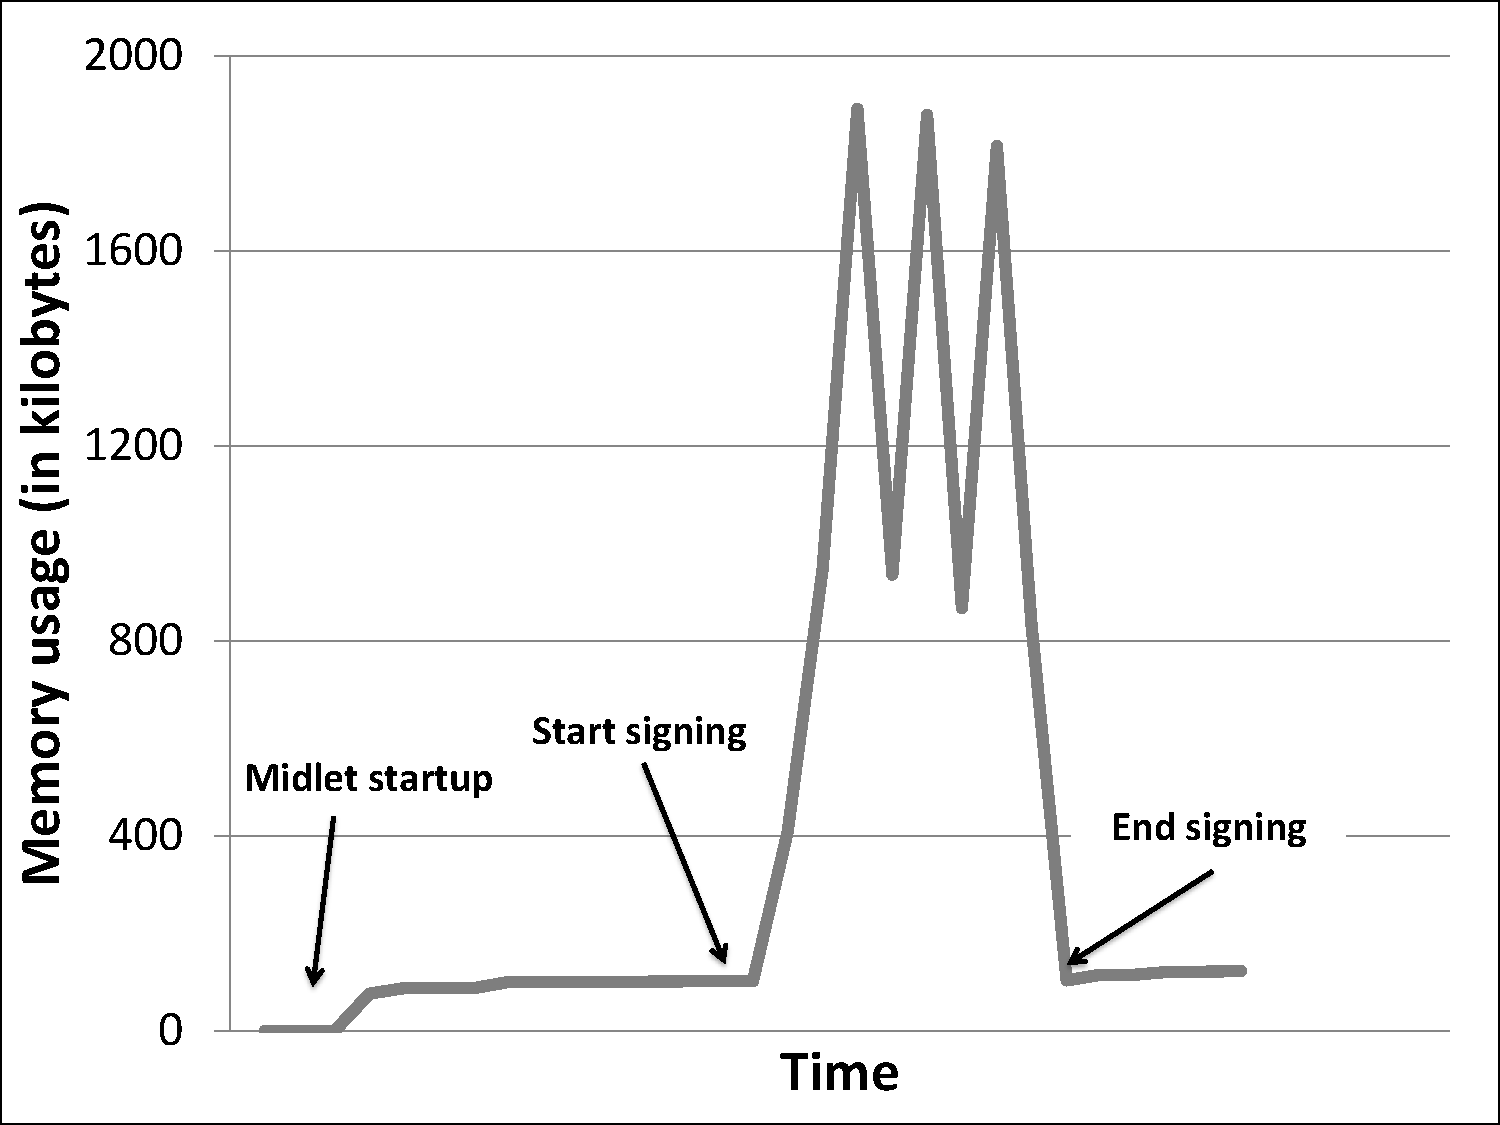
\includegraphics[width=7cm]{immagini/MemoryECDSA.pdf}\\
  \caption{Memory usage profile of \textbf{ECDSA} when processing a 160-bit signature}
  \label{fig:MemoryECDSA}
\end{center}
\end{figure}

\begin{figure}[ht]
\begin{center}
%%%  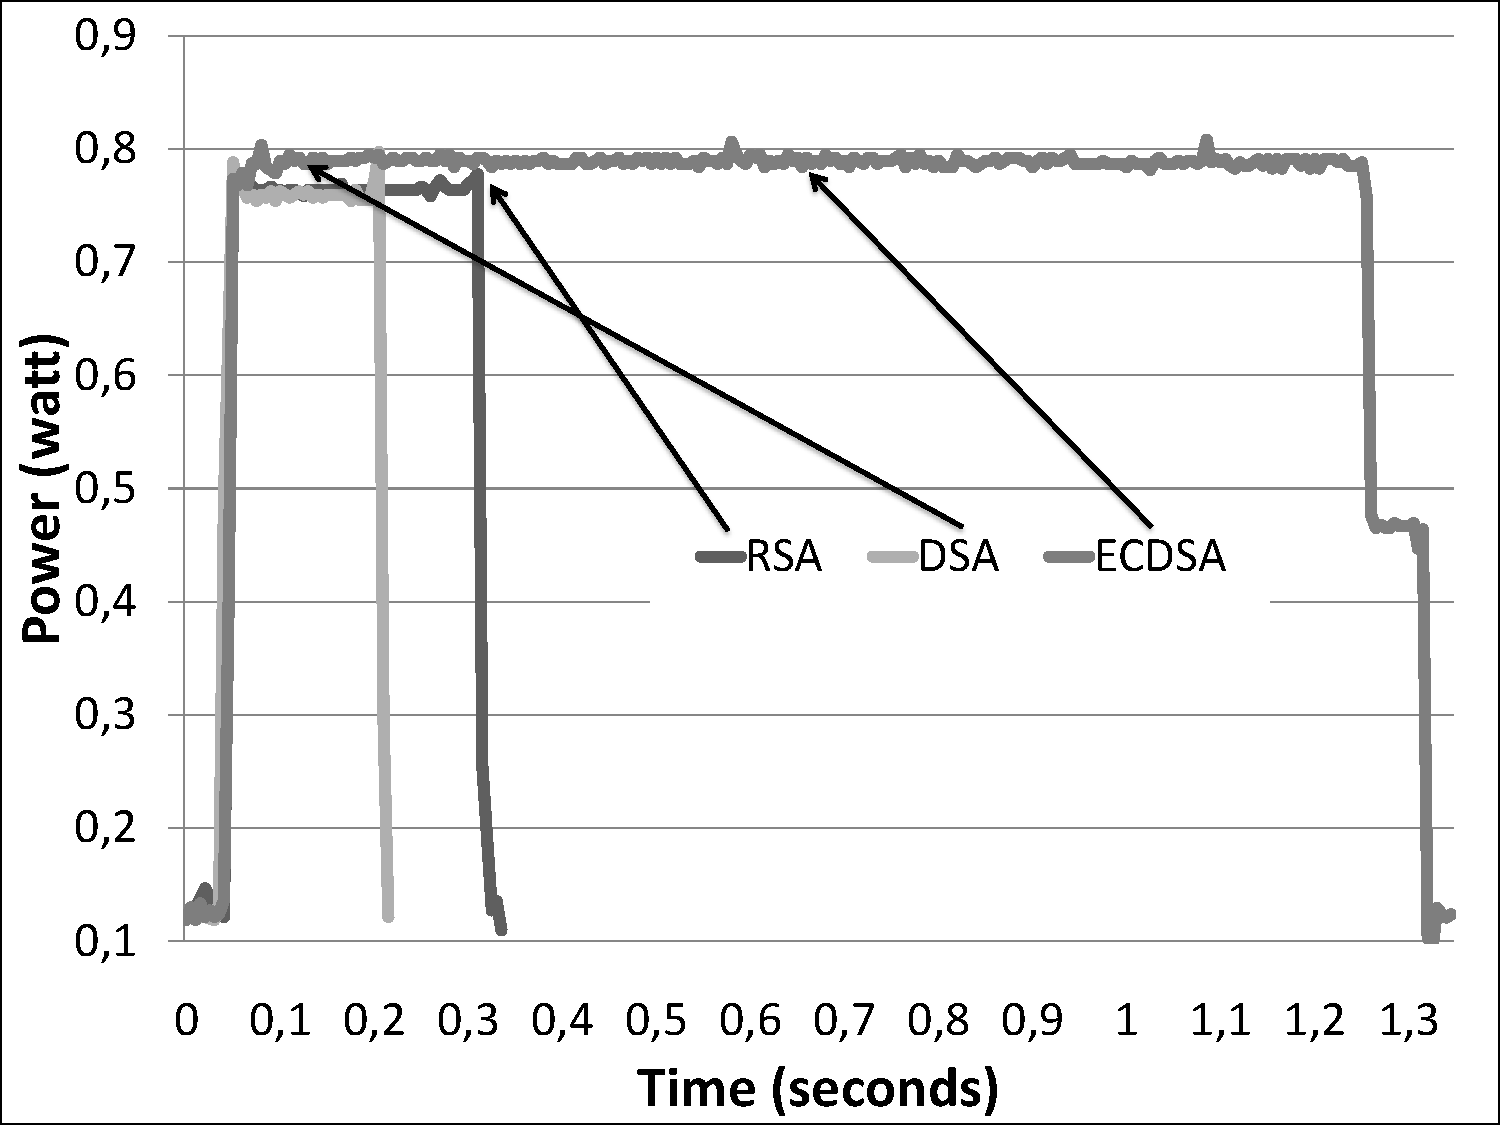
\includegraphics[width=9cm]{immagini/Power.eps}\\
  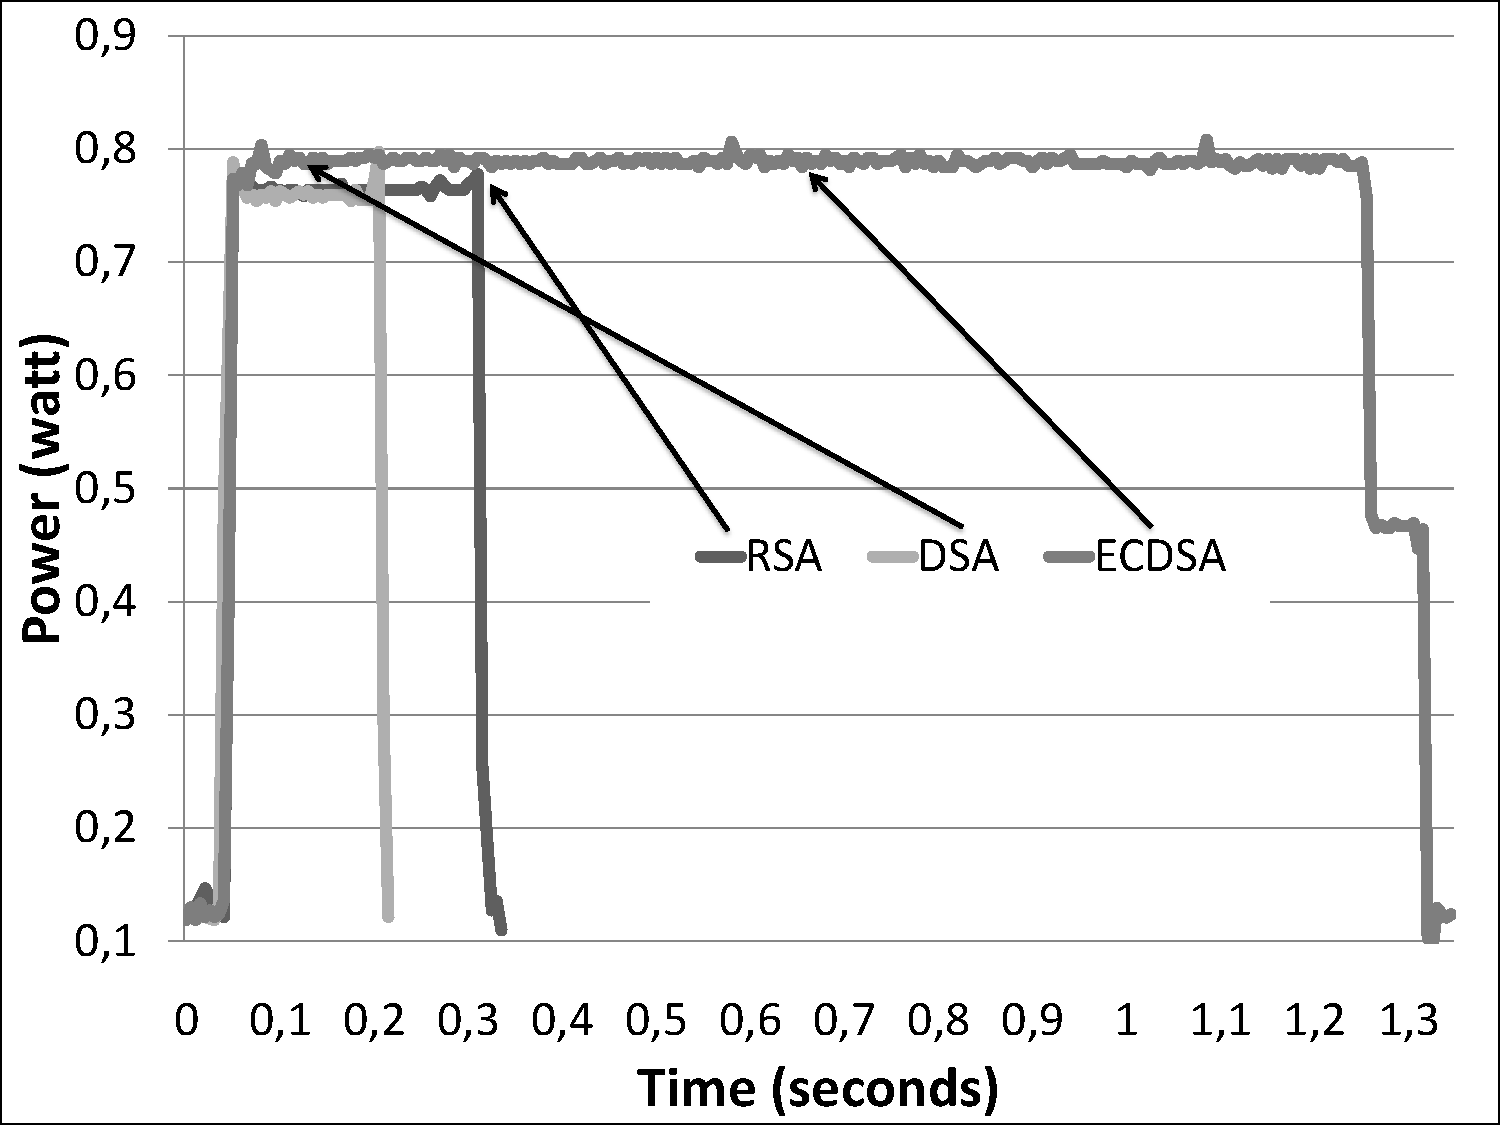
\includegraphics[width=7cm]{immagini/Power.pdf}\\
  \caption{N95-8GB power consumption when signing a message using a $1.024$ bits key}
  \label{fig:N95Power}
\end{center}
\end{figure}


% The Table \ref{table:N95FirstVerify} show the time spent for the first signature verification on the N95-8GB.

% \begin{table}[ht]
% \caption{N95-8GB first signature verification}
% \centering % used for centering table
% \begin{tabular}{c|c c c} % centered columns (4 columns)
% \hline\hline %inserts double horizontal lines
% Key strength (bit) & RSA (ms) & DSA (ms)& ECDSA(ms) \\ [0.5ex] % inserts table
% %heading
% \hline\hline % inserts single horizontal line
% 512  & 61   & 246  & 1088  \\ % inserting body of the table
% 704  & 116  & 257  & 1398  \\
% 1024 & 136  & 446  & 2432  \\
% 1536 & 147  & -    & 3548  \\
% 2048 & 151  & -    & 4910  \\
% 3072 & 171  & -    & 7262  \\ [1ex] % [1ex] adds vertical space
% \hline %inserts single line
% \end{tabular}
% \label{table:N95FirstVerify} % is used to refer this table in the text
% \end{table}

% Time reported in Table \ref{table:N95FirstVerify} are still bigger than the medium as in the case of the signature process.

%\subsection{Memory Efficiency}

\subsection{Energy Efficiency}
A cryptosystem running on a mobile device may put its CPU on a heavy load and significantly drain the underlying battery, as witnessed by several contributions in this field \citep{Potlapally06,KimHL06,wander2005energy}. This consumption is proportional to the execution time of the cryptosystem and to the complexity of the involved cryptographic operations. The expectations are that performing a signature using ECDSA instead of RSA or DSA is less energy-expensive because this cryptosystem uses simpler operations and shorter keys. When performing a signature verification, it is also expected that RSA is much more energy saving than DSA and ECDSA since it is able to perform this operation faster.

Starting from these premises,  the energy consumption of the three cryptosystems was profiled when performing a signature and a verification on a message using a security level equivalent to $1.024$ bits RSA key.

The measurements have been taken by running the SEESMS client application on a Nokia N95-8GB using the Nokia Energy Profiler tool. Figure \ref{fig:N95Power} shows the energy required to perform one signature using the cryptosystems currently supported by SEESMS. Despite the expectations, the energy cost of the ECDSA algorithm ($\sim0,79$ Watts) is higher than RSA and DSA algorithms ($\sim0,76$ Watts). Moreover, since ECDSA execution time is longer than the other two algorithms, its overall energy consumption ($\sim1,04$ Joule) results to be larger than RSA ($\sim0,25$ Joule) and DSA ($\sim0,15$ Joule).
\newpage


Figure \ref{fig:N95PowerVerify} shows the energy consumption of one signature verifications using the supported cryptosystems with a key strength of $1.024$ bits. Even in this case the Watts consumption for the ECDSA algorithm ($\sim 0,77$ Watts) is higher than RSA ($\sim0.70$ Watts) and DSA algorithms ($\sim 0,68$ Watts). Moreover, it is interesting to observe that the overall energy consumption of the ECDSA algorithm ($\sim1,23$ Joule) is higher than RSA ($\sim 0,03$ Joule) and DSA ($\sim0,20$ Joule), due to its longer verification time.

\begin{figure}[ht]
\begin{center}
%%%  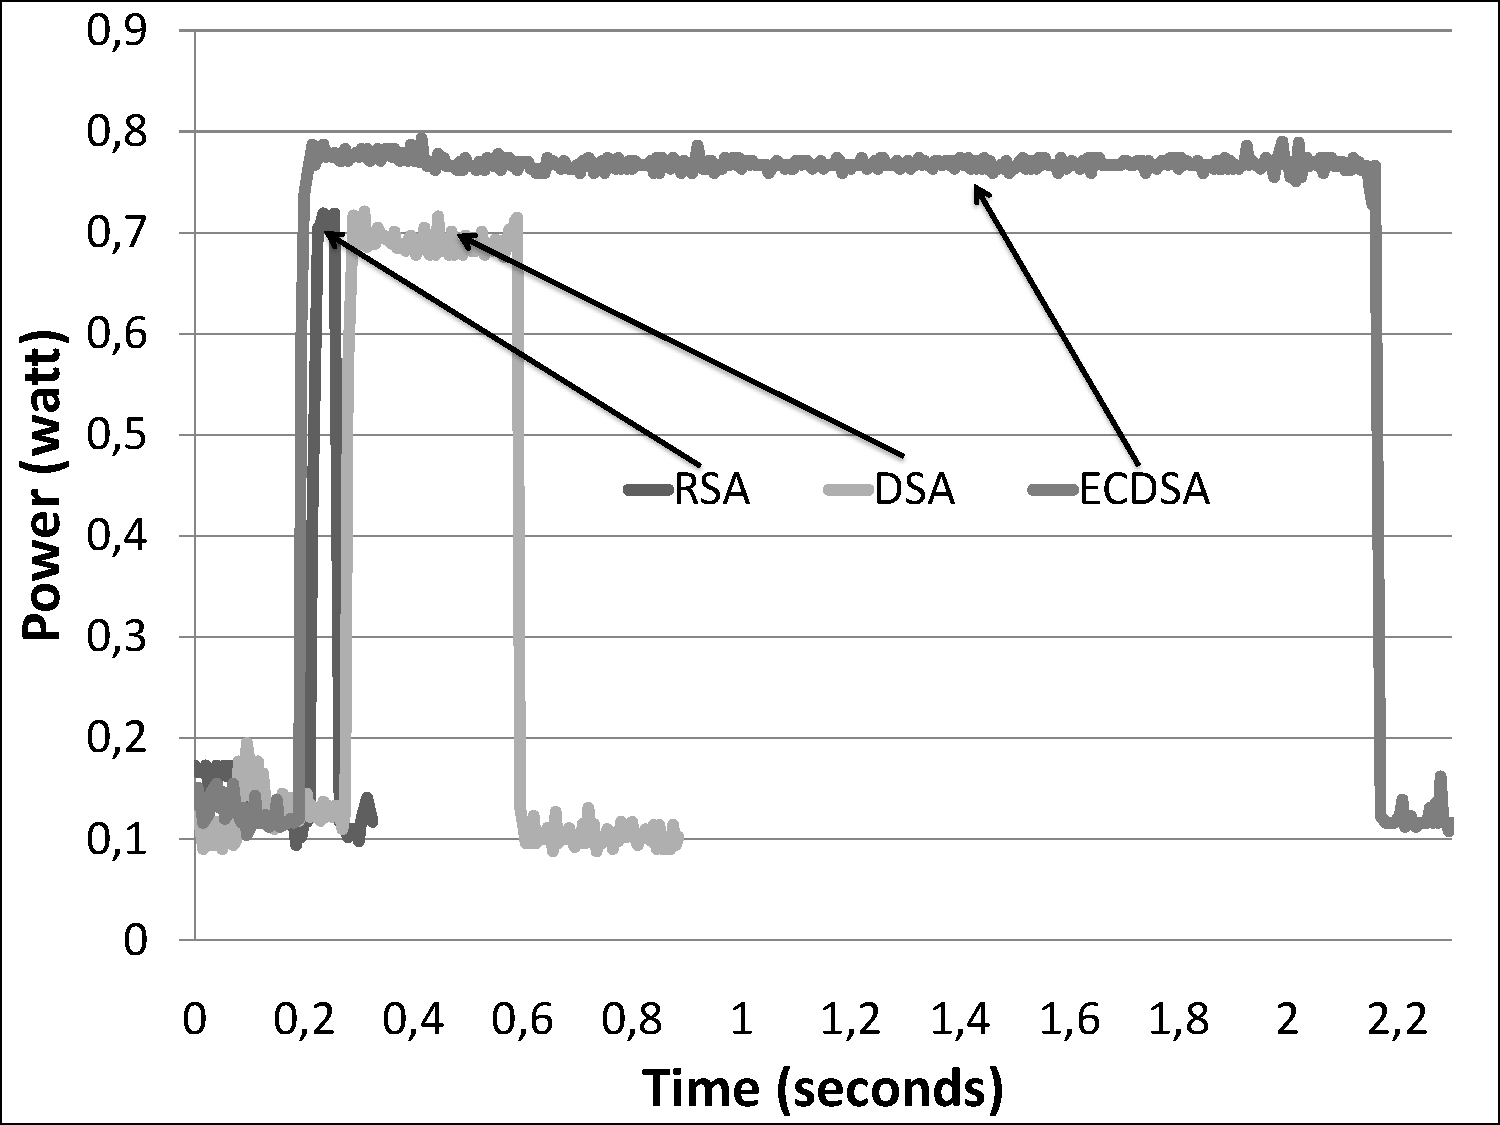
\includegraphics[width=9cm]{immagini/N95PowerVerify.eps}\\
  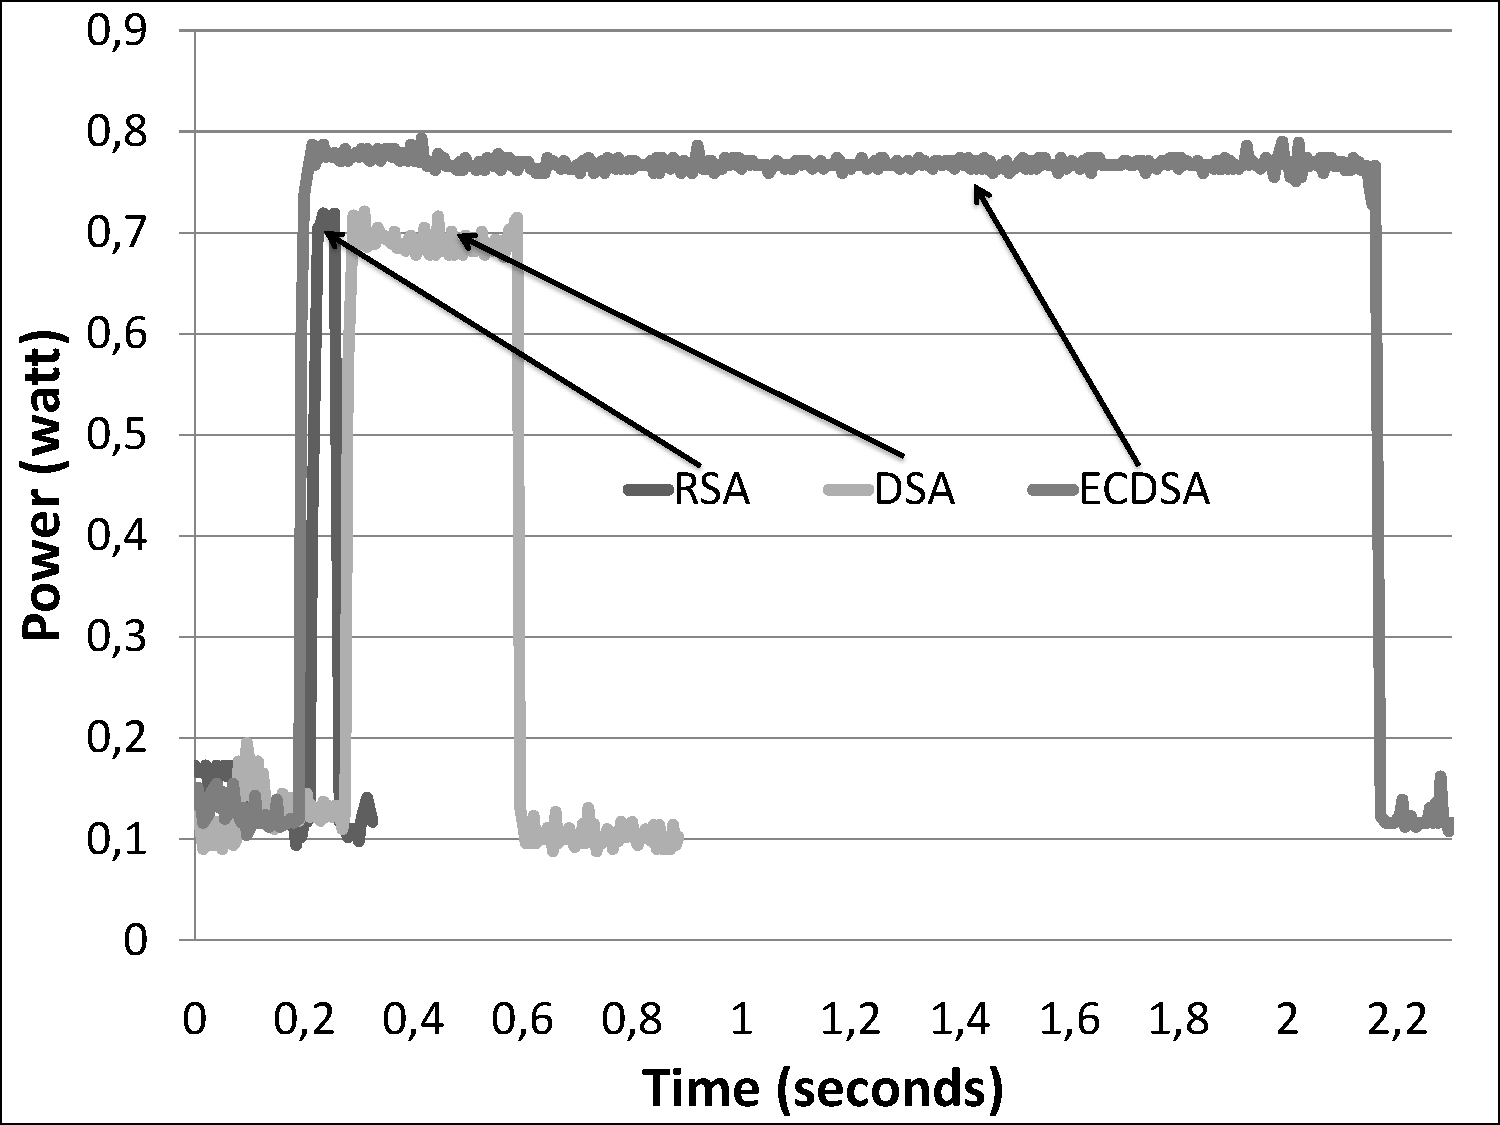
\includegraphics[width=7cm]{immagini/N95PowerVerify.pdf}\\
  \caption{N95-8GB power consumption when verifying a message using a $1.024$ bits key}
  \label{fig:N95PowerVerify}
\end{center}
\end{figure}


\section{Optimization}
The poor overall performance of ECDSA and its suspicious memory usage graph motivated us in investigating the quality of the implementation we have been using for this algorithm. The purpose of this investigation was to understand if these bad performance were due to algorithmic reasons or to some implementation defects. In this section, we further profile the inner behavior of the ECDSA implementation we have been using, we pinpoint some serious performance issues and, finally, we experiment with several optimizing algorithmic techniques in order to improve its speed. The discussion is organized according to the chronological order we have followed when trying the different optimizations, with all the succeeding optimization techniques applied in an incremental way over the original ECDSA and, in some case, RSA cryptosystems.


%describe the optimizations applied to the ECDSA implementation starting from those related to memory management. We then describe an other known algorithm we implemented to speedup the overall ECDSA performance. We measured the efficiency of our implementation and compared the results with those described in Section \ref{sec:experimental results} and, as we will show, a decrease of about $95\%$ on the total time required to produce an ECDSA signature.
%

%This further step was motivated by other two factors. First, the fact that RSA overcome ECDSA in performance contradicts the several theoretical results which state the contrary. Second, we observed this inversion in performance with respect to RSA only for the java implementation of ECDSA on mobile devices. 

%
%Indeed, we tested the same Bouncy Castle ECDSA implementation on desktop PC and several \emph{C} language implementation on both mobile and desktop PC platform and ECDSA registered better performance with respect to RSA.



%As we seen in the previous sections, the ECDSA memory usage graph revealed a strange behavior consisting of many repeated memory allocation and deallocation.

% We investigated the performance of Java implementations of most
% popular cryptosystems on mobile devices, (RSA\citep{Rivest78},
% DSA\citep{NISTDSA} and ECDSA\citep{ECDSA}). In order to obtain a better
% evaluation among the cryptosystems, all implementations come from the
% same library, Bouncy Castle\citep{Bouncy}. Moreover this is the only
% known open source library containing the required cryptosystems
% implementations.

% This investigation was motivated from the results of previous work
% (SEESMS\citep{SEESMS2010}), where the ECDSA signature performances were
% worse than those of RSA for small keys (less than 2048 bit). The fact
% that RSA uses larger integers and must perform a slow modular
% exponentiation, should make any private key operation slower than
% private key operation in ECDSA for equivalent security level.

\subsection{Optimizing Memory Usage}
\label{subsec:optmem}
% In particular we found that, inside the scalar multiplication, the
% most time consuming part is the one which uses prime field arithmetic
% in which field elements are represented by means of big
% integers.

In our previous experiments on the memory usage of ECDSA (see, e.g., Figure \ref{fig:MemoryECDSA}), we have observed that there may be some issues with the way this cryptosystem manages its own memory. Namely, we have seen that ECDSA requires about $100$ times the memory used by the equivalent RSA implementation. Moreover, we noticed that during its execution, the algorithm performs many memory allocations/deallocations. Indeed, this behavior may have a strong negative influence on the performance of the algorithm because of the time overhead required to perform memory related operations.

Starting from these observations, we focused our attention on the data types used by the ECDSA implementation available with the Bouncy Castle library, and on the way they are used in the implementation.  A quick analysis revealed that the most resource-consuming data type used by this algorithm is the one implemented by the {\tt BigInteger} class, which serves to store an integer number of arbitrary length. The weak point of this data type is that is implemented as an {\em Immutable} object, that is: every time an instance of this object has to change the value it represents, a new instance has to be created to store the new value.  It is interesting to note that the original {\tt BigInteger} implementation available with the J2SE framework relies on the existence of an additional {\tt BigInteger} implementation which is {\em mutable}. Instead, the J2ME framework does not implement the {\tt BigInteger} class, in fact it is provided by the BC library.

As a confirmation of our intuition, we have seen that during the processing of a $160$ bit based signature on a mobile device, ECDSA required the allocation of approximately $100.000$ {\tt BigInteger} objects. Instead, by running the same code on a desktop environment and using the native J2SE {\tt BigInteger} implementation, we have seen that the overall number of allocations dropped to $3.700$.

\begin{figure}[ht]
\begin{center}
  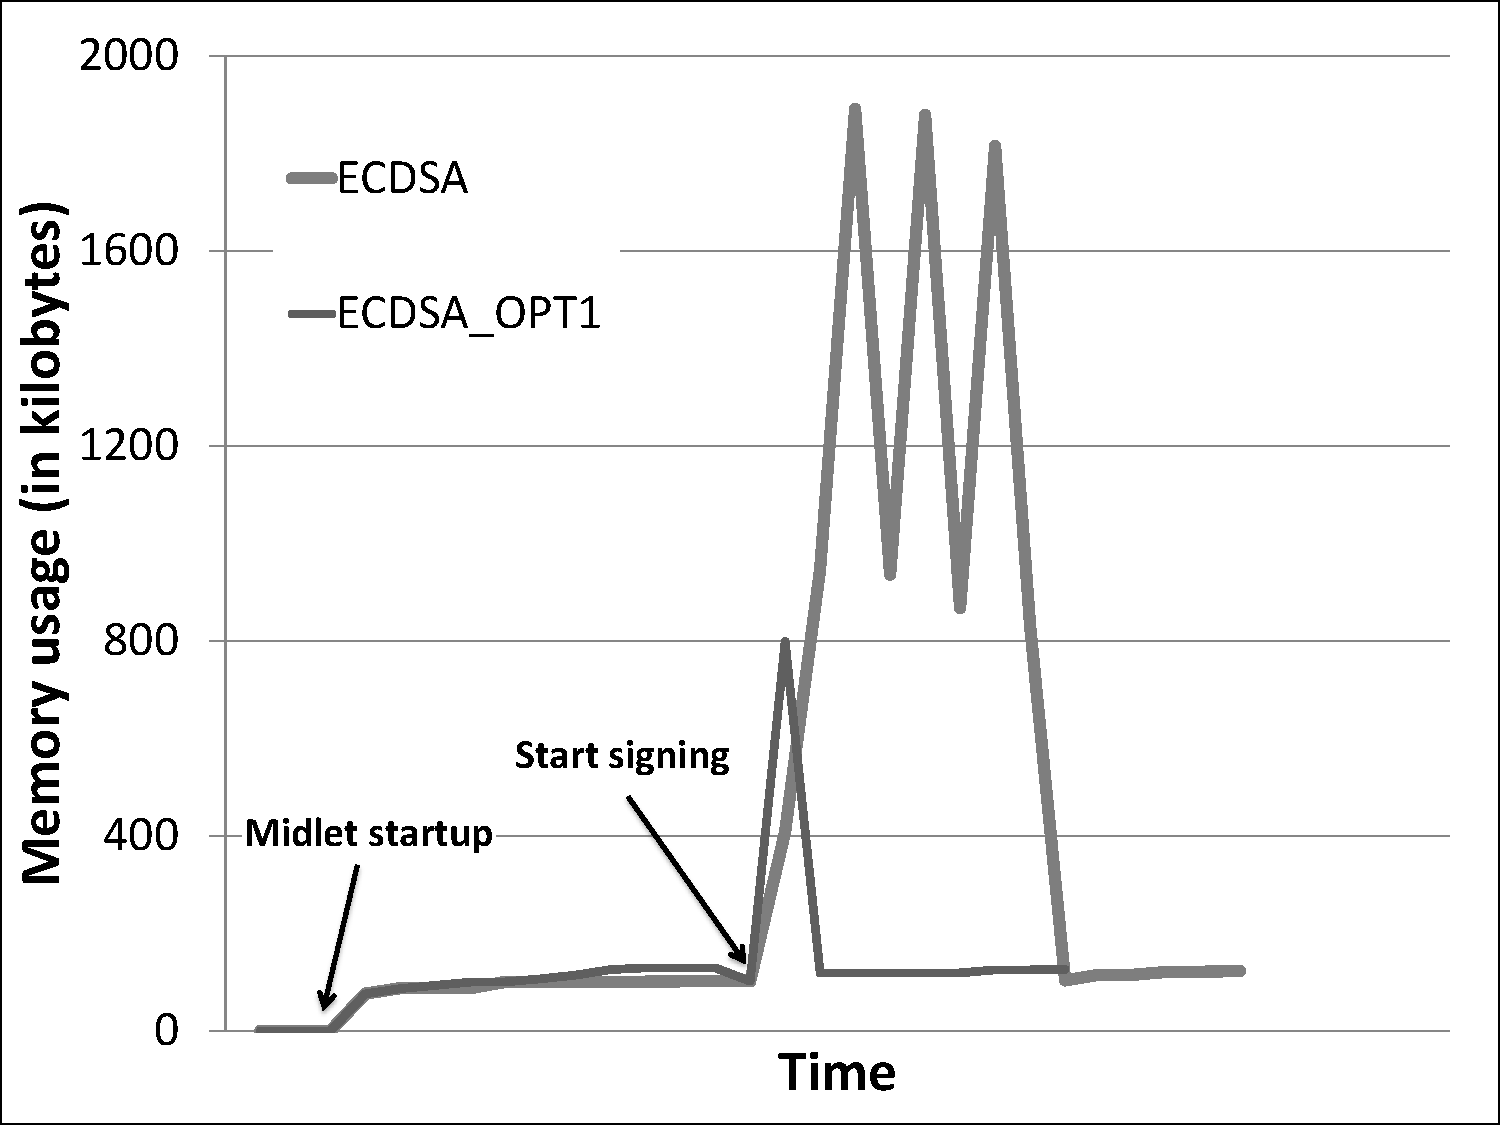
\includegraphics[width=7cm]{immagini/MemoryECDSA_OPT1.pdf}\\
  \caption{Memory usage profile of \textbf{ECDSA} and \textbf{ECDSA\_OPT1} when processing a 160-bit signature}
  \label{fig:MemoryECDSA_OPT1}
\end{center}
\end{figure}

We then optimized \textbf{ECDSA}  by replacing the original {\tt BigInteger} class coming with BC with a porting of the mutable one available with the J2SE framework. The resulting code, which we called \textbf{ECDSA\_OPT1}, exhibits a much more regular memory usage pattern than \textbf{ECDSA} and requires about 800 kbytes instead of 5.400 kbytes, as shown in Figure \ref{fig:MemoryECDSA_OPT1}. This optimization has also a significant impact on the running times of the algorithms, which are now about six times faster than the original implementation (see Table \ref{table:BCJ2SE-BigVSJ2SEBIG} ). We performed the same optimization on the RSA implementation by replacing the original {\tt BigInteger} class with the new one. The resulting implementation, \textbf{RSA\_OPT1}, is about the $30\%$ faster than the original RSA implementation.

% Memory profiling revealed an abnormal of allocation and
% deallocation of Big Integer during executions. For example, during a
% 160-bit digital signature, the wireless toolkit memory profiler
% counted about 100.000 big integer object allocated.

% We then profiled the algorithms on desktop in J2SE environment. This code differs from that mobile only for the implementation of the Big Integer class, where in the first case are those of the standard version (J2SE) while in the latter are those implemented ad hoc for the mobile by Bouncy Castle. The results showed that in the desktop environment the number of big integer allocated was much lower than those used by the mobile version, about xxxx versus 100,000.

% In order to improve ECDSA performance on mobile devices, we optimized
% the code of the Bouncy Castle big integer implementation using the
% J2SE big integer implementation as a reference. The optimization
% applied to the Big Integer class produced a great reduction in big
% integer allocation (about 3.700 versus 100.000). Moreover as shown in
% Table \ref{table:BCJ2SE-BigVSJ2SEBIG} the time required for a digital
% signature on a real device is about 5 time faster with respect to the
% Bouncy Castle-only implementation.

\begin{table}[ht]
\caption{ECDSA and RSA signature times (in ms) on an N95-8GB device, with increasing security levels. ECDSA key sizes are reported, together with their RSA security equivalent sizes.}
\centering % used for centering table
\begin{tabular}{|c|c|c|c|c|} % centered columns (4 columns)
\hline\hline %inserts double horizontal lines
Bit per key & ECDSA & ECDSA\_OPT1 & RSA & RSA\_OPT1\\
%heading
\hline\hline % inserts single horizontal line
112 (512) & 461 & 112 & 49 & 27      \\
128 (704) & 596	& 132 & 86 & 63      \\
160 (1.024) & 1.020 & 184 & 236 & 164   \\
192 (1.536) & 1.651 & 332 & 735 & 499   \\
224 (2.408) & 2.343 & 481 & 1.666 & 1.127 \\
256 (3.072) & 3.096 & 568 & 5.503 & 3.588 \\ % [1ex] adds vertical space
\hline %inserts single line
\end{tabular}
\label{table:BCJ2SE-BigVSJ2SEBIG} % is used to refer this table in the text
\end{table}

% We repeated the test on the memory consumption of the ECDSA algorithm using our bin integers implementation and we obtained a lower growing curve as shown in Figure \ref{fig:MemoryECDSA_OPT1}.




\subsection{Optimizing Running Times}
\label{Speedup}
Despite the memory optimizations described in Section \ref{subsec:optmem}, \textbf{ECDSA\_OPT1} still remains significantly slower than \textbf{RSA} when used to perform digital signatures with large keys. A careful profiling of this algorithm revealed that, in this case, it spends more than the $95\%$ of its execution time to perform \emph{scalar multiplications}, i.e., the product of a big scalar value and the representation of a curve point in affine coordinates. According to \citet{Menezes}, given  a scalar $k = \{k_0, k_1, \ldots, k_{m-1}\}$, this operation can be defined as:

\begin{center}
$kP = \sum_{i=0}^{m-1} k_i(2^iP)$
\end{center}

Considering that the expected number of ones in the binary representation of $k$ is about $m/2$\footnote{In our context $k$ is the private key.}, the expected number of operations needed to carry out a scalar multiplication is approximately $m/2$ point additions and $m$ point doublings.

A common approach to the optimization of this operations uses, first, the Non-Adjacent Form \citep{Menezes} (NAF) technique to minimize the number of points additions to do, and then, the Fixed-base Windowing method \citep{BrownHLM01} to precalculate some of the intermediate values required by a scalar multiplication.

\subsubsection{The NAF algorithm}
According to \citet{Menezes}, a NAF of a scalar \emph{k} is a \emph{signed digit representation} in the form of $k = \sum_{i=0}^{l-1} k_i2^i$ where $k_i \in \{0,\pm1\}$, $k_{l-1} \neq 0$, and no two consecutive digits $k_i$ are nonzero. The \emph{length} of the NAF is \emph{l}.

For every integer positive $k$, the NAF expression has the following properties which can be exploited to improve the performance of the elliptic curve scalar multiplier:

\begin{enumerate}
  \item $k$ has a unique NAF denoted NAF($k$).
  \item NAF($k$) has the fewest nonzero digits of any signed digit representation of $k$.
  \item The length of NAF($k$) is at most one more than the length of the binary representation of $k$.
  \item If the length of NAF($k$) is $l$, then $2^l/3 < k < 2^{l+1}/3$.
  \item The average density of nonzero digits among all NAFs of length $l$ is approximately $1/3$.
\end{enumerate}

NAF($k$) can be efficiently computed using an algorithm that generates the digits of the NAF($k$) by repeatedly dividing $k$ by 2.

% \begin{algorithm}
% \caption{Computing the NAF of a positive integer}
% \label{NAF}
% \begin{algorithmic}[1]
% \REQUIRE A positive integer $k$
% \ENSURE NAF($k$)
% \STATE $i \leftarrow 0$
% \WHILE{$k \geq 1$}
% \IF{$k$ is odd}
% \STATE $k_i\leftarrow 2-(k$ mod $4)$
% \STATE $k \leftarrow k-k_i$
% \ELSE
% \STATE $k_i \leftarrow 0$
% \ENDIF
% \STATE $k \leftarrow k/2$
% \STATE $i \leftarrow i+1$
% \ENDWHILE
% \RETURN ($k_{i-1}, k_{i-2}, \ldots, k_1, k_0$)
% \end{algorithmic}
% \end{algorithm}

NAF can be defined in a more general way using a parameter $w$ (window) and hence processing $w$ digits of $k$ at time.

Let $w \geq 2$ be a positive integer. A \emph{width-w} NAF of a scalar \emph{k} is a \emph{signed digit representation} in the form of $k = \sum_{i=0}^{l-1} k_i2^i$ where each nonzero coefficient $|k_i|$ is odd, $|k_i| < 2^{w-1}$, $k_{l-1} \neq 0$, and at most one of any \emph{w} consecutive digits is nonzero. The \emph{length} of the \emph{width-w} NAF is \emph{l}.

Let k be a positive integer.
\begin{enumerate}
  \item $k$ has a unique \emph{width-w} NAF denoted $NAF_w(k$).
  \item $NAF_2(k) = NAF(k)$.
  \item The length of $NAF_w(k)$ is at most one more than the length of the binary representation of $k$.
  \item The average density of nonzero digits among all \emph{width-w} NAFs of length $l$ is approximately 1/($w$+1).
\end{enumerate}

\subsubsection{The Fixed-base Windowing method}
The \emph{fixed-base windowing} method for point multiplication exploits the fact that if the point $P$ is known (as in the case of ECDSA) and some storage is available, then the point multiplication can be spedeed up by precomputing some data which depends only on $P$. For example, if the points $2P$, $2^2P$,  \ldots, $2^{m-1}P$ are precomputed, then the expected time required for the scalar multiplier would be $m/2$ additions.

Let $(k_{d-1}, \ldots, k_1, k_0)_{2^w}$ be the $2^w$-ary representation of $k$, where $d=\lceil m/w \rceil$, and let $Q_j = \sum_{i:k_i=j} 2^{wi}P$. Then

\medskip


 $kP = \sum_{i=0}^{d-1}k_i(2^{wi}P) = \sum_{j=1}^{2^w-1}(j\sum_{i:k_i=j}2^{wi}P) = \sum_{j=1}^{2^w-1}jQ_j$.
\medskip

Hence
\begin{equation}\label{KP}
kP = Q_{2^w-1} + (Q_{2^w-1}+Q_{2^w-2}) + \dots + (Q_{2^w-1}+Q_{2^w-2}+\dots+Q_1).
\end{equation}

The \emph{fixed-base windowing method} is based on (\ref{KP}) and its expected running time is approximately $((d(2^w-1)/2^w-1)+(2^w-2))A$.

% \begin{algorithm}
% \caption{Fixed-base windowing method for point multiplication}
% \label{FBWM}
% \begin{algorithmic}[1]
% \REQUIRE Windows width $w$, $d = \lceil m/w \rceil$, $(k_{d-1}, \ldots, k_1, k_0)_{2^w}$, $P \in E(\mathbb{F}_p)$.
% \ENSURE $kP$
% \STATE \emph{Precomputation.} Compute $P_i = 2^{wi}P, 0\leq i\leq d-1$
% \STATE $A \leftarrow O, B \leftarrow O,$
% \FOR {$j = 2^w-1$ downto 1}
% \STATE For each $i$ for which $k_i = j$ do: $B \leftarrow B+P_i.$   \{Add $Q_j$ to $B$\}
% \STATE $A \leftarrow A + B$
% \ENDFOR
% \RETURN ($A$)
% \end{algorithmic}
% \end{algorithm}

% \Begin{table}[ht]
% \caption{Spatial requirements for the fixed-base window method. $w$ is the window width while $S$ denotes the number of points stored by the precomputation phase.}
% \centering % used for centering table
% \begin{tabular}{|c|c|} % centered columns (4 columns)
% \hline\hline %inserts double horizontal lines
%  Precomputation size for the &  \\
%  Fixed-base window method & S \\
% %heading
% \hline\hline % inserts single horizontal line
% $w = 2$ & 95	   \\
% $w = 3$ & 63	   \\
% $w = 4$ & 47	  \\
% $w = 5$ & 38	  \\
% $w = 6$ & 31	  \\
% $w = 7$ & 27	  \\ % [1ex] adds vertical space
% $w = 8$ & 23	  \\
% \hline %inserts single line
% \end{tabular}
% \label{table:SpacePrecomp} % is used to refer this table in the text
% \end{table}



\begin{table}[hb]
\caption{Overall number of ECPoint objects initializations, additions and doublings required by \textbf{ECDSA} and \textbf{ECDSA\_OPT2}}
\centering % used for centering table
\begin{tabular}{|c|c|c|} % centered columns (4 columns)
\hline\hline %inserts double horizontal lines
 & ECDSA & ECDSA\_OPT2 \\
%heading
\hline\hline % inserts single horizontal line
ECPoint Init & 239 & 54 \\
Addition     & 35  & 29 \\
Doubling   & 159 & 0 \\
\hline %inserts single line
\end{tabular}
\label{table:CountOps} % is used to refer this table in the text
\end{table}

\subsubsection{Experimental Results}
We implemented another variant of \textbf{ECDSA}, called \textbf{ECDSA\_OPT2}, that uses the window-NAF coding for the scalar $k$ and the fixed-base windowing method. The size $w$ of the window has been chosen in such a way to optimize the trade-off between the number of multiplications saved by precomputation and the number of fields operations required to perform it. In Table \ref{table:CountOps} we report some statistics about the improvement on the overall number of operations to be performed when producing an ECDSA signature using \textbf{ECDSA\_OPT2} rather than \textbf{ECDSA}. This improvement affects also the performance of \textbf{ECDSA\_OPT2} which results to be much faster than \textbf{ECDSA\_OPT1}, as clearly visible in 
Table \ref{table:BCJ2SE-BigVSJ2SEBIG_Pre}: the performance improvement is noteworthy as this new variant requires less than the $10\%$ of the time required by \textbf{ECDSA\_OPT1} and about the $2\%$ of the time required by \textbf{ECDSA}. We also observe a significant improvement on the memory usage of \textbf{ECDSA\_OPT2}, which is approximately the  $10\%$ of the memory used by \textbf{ECDSA\_OPT1}  (see Figure \ref{fig:MemoryECDSA_OPT2}).

\begin{table}[ht]
\caption{ECDSA signature times (in ms) on an N95-8GB device}
\centering % used for centering table
\begin{tabular}{|c|c|c|c|} % centered columns (4 columns)
\hline\hline %inserts double horizontal lines
Bit per key & ECDSA & ECDSA\_OPT1 & ECDSA\_OPT2 \\
%heading
\hline\hline % inserts single horizontal line

112  & 461 & 112 & 17  \\
128  & 596	& 132 & 24  \\
160 & 1.020 & 184 & 38 \\
192  & 1.651 & 332 & 43 \\
224  & 2.343 & 481 & 46 \\
256  & 3.096 & 568 & 61 \\ % [1ex] adds vertical space
\hline %inserts single line
\end{tabular}
\label{table:BCJ2SE-BigVSJ2SEBIG_Pre} % is used to refer this table in the text
\end{table}

\begin{figure}[ht]
\begin{center}
  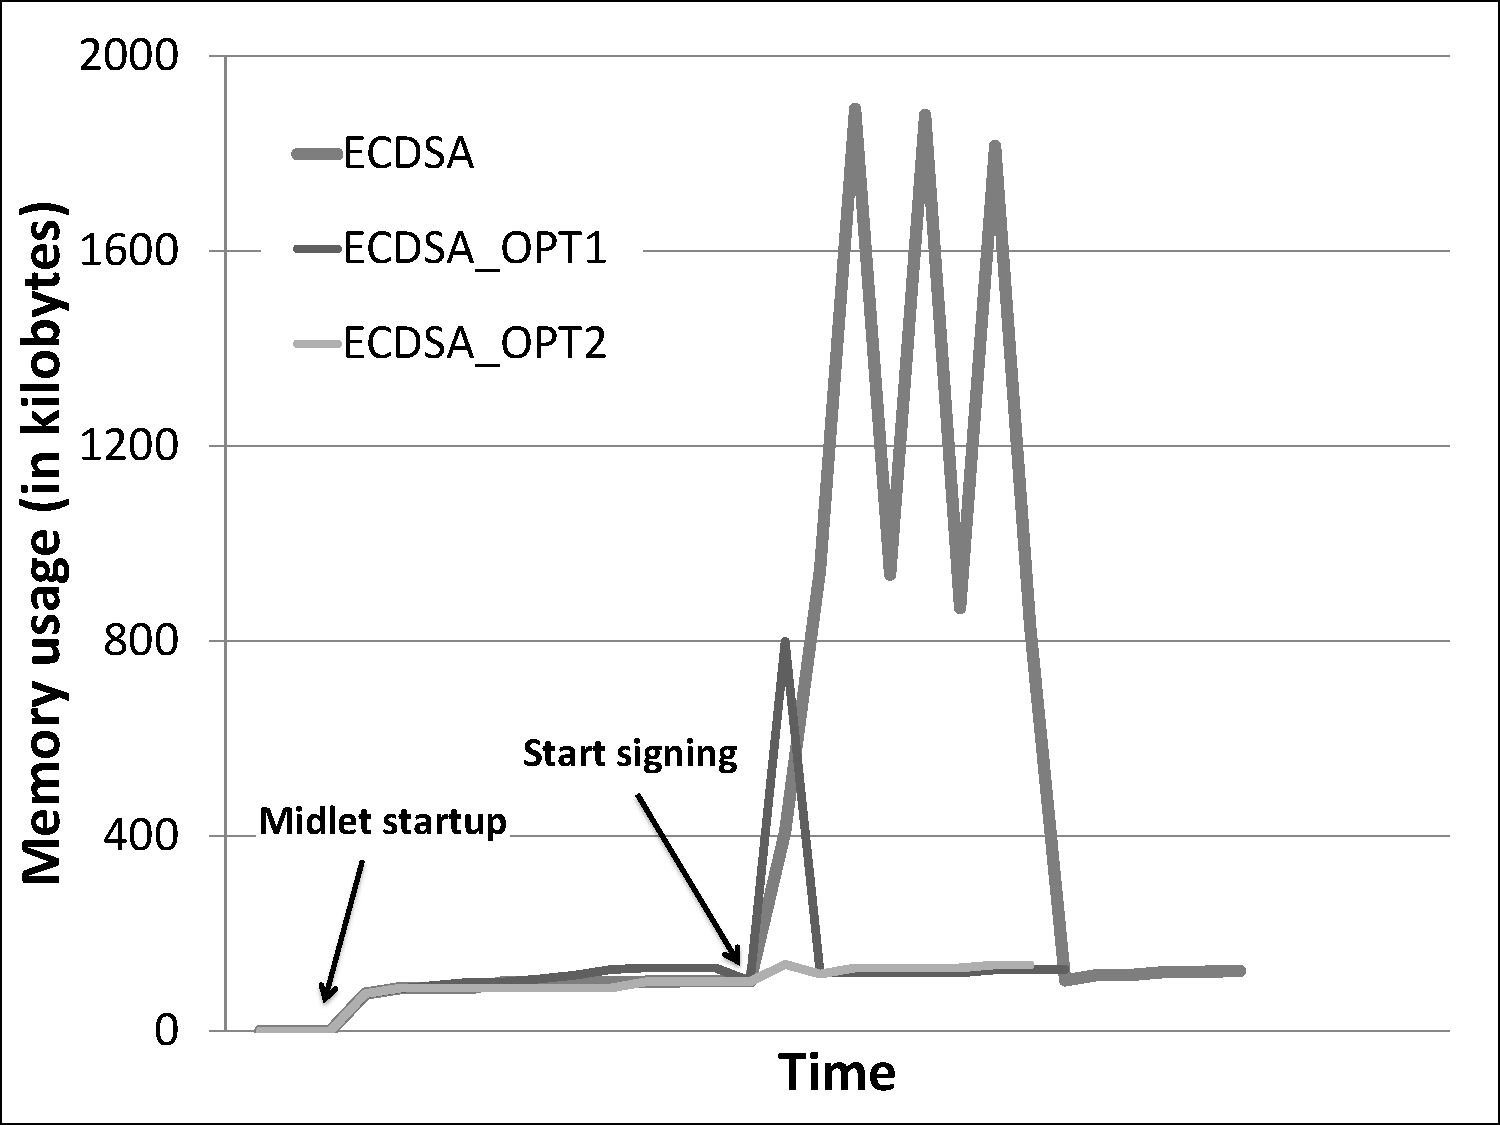
\includegraphics[width=6.8cm]{immagini/MemoryECDSA_OPT2.pdf}\\
  \caption{Memory usage profile of \textbf{ECDSA}, \textbf{ECDSA\_OPT1} and \textbf{ECDSA\_OPT2} when processing a 160-bit signature}
  \label{fig:MemoryECDSA_OPT2}
\end{center}
\end{figure}





\subsection{Overall Experimental Results}

The several optimizations discussed so far led to \textbf{ECDSA\_OPT2}, a variant of \textbf{ECDSA} that exhibits a significant performance improvement with respect to the original implementation. We have been able to improve as well the performance of \textbf{RSA} through the implementation of \textbf{RSA\_OPT1}, a variant of the original implementation that uses the optimized version of the {\tt BigInteger} data type. We now turn our attention to the way these new implementations compare to each other from differ viewpoints. Concerning time performance, \textbf{ECDSA\_OPT2} is extremely more efficient than \textbf{ECDSA} when signing messages and performs much better than the RSA-based implementations, also for short keys. This is shown in Figure \ref{fig:Firme_OPT1_OPT2}. We also observed a significant speed-up of \textbf{ECDSA\_OPT2} over \textbf{ECDSA} when verifying the signature of a message, as visible in Figure  \ref{fig:Verifiche_OPT1_OPT2}. In this case, the RSA-based implementations remain the fastest cryptosystems, however \textbf{ECDSA\_OPT2} exhibits approximately the same order of growth. Concerning memory usage, the space requirements of \textbf{ECDSA\_OPT2} are slightly higher than those of \textbf{RSA\_OPT1} because of the overhead to be paid for precalculating and storing in memory  the points to be used by the \emph{fixed-base windowing} method (see Figure \ref{fig:MemoryRSA1ECDSA2}). 

Finally, we briefly discuss the impact of these optimizations on the overall amount of energy consumed by the considered algorithms. The Watt consumption per second is almost unaffected by all the optimizations we have introduced however, the shorter execution times imply smaller amount of energies to be spent for performing the signature and verification operations, as it can be seen in Figures \ref{fig:N95Power_OPT} and \ref{fig:N95PowerVerify_OPT}. Anyway, the energy cost of these operations does not have a significant impact on the typical battery life of a smartphone device. 

%\clearpage 

 \begin{figure}[h]
\begin{center}
  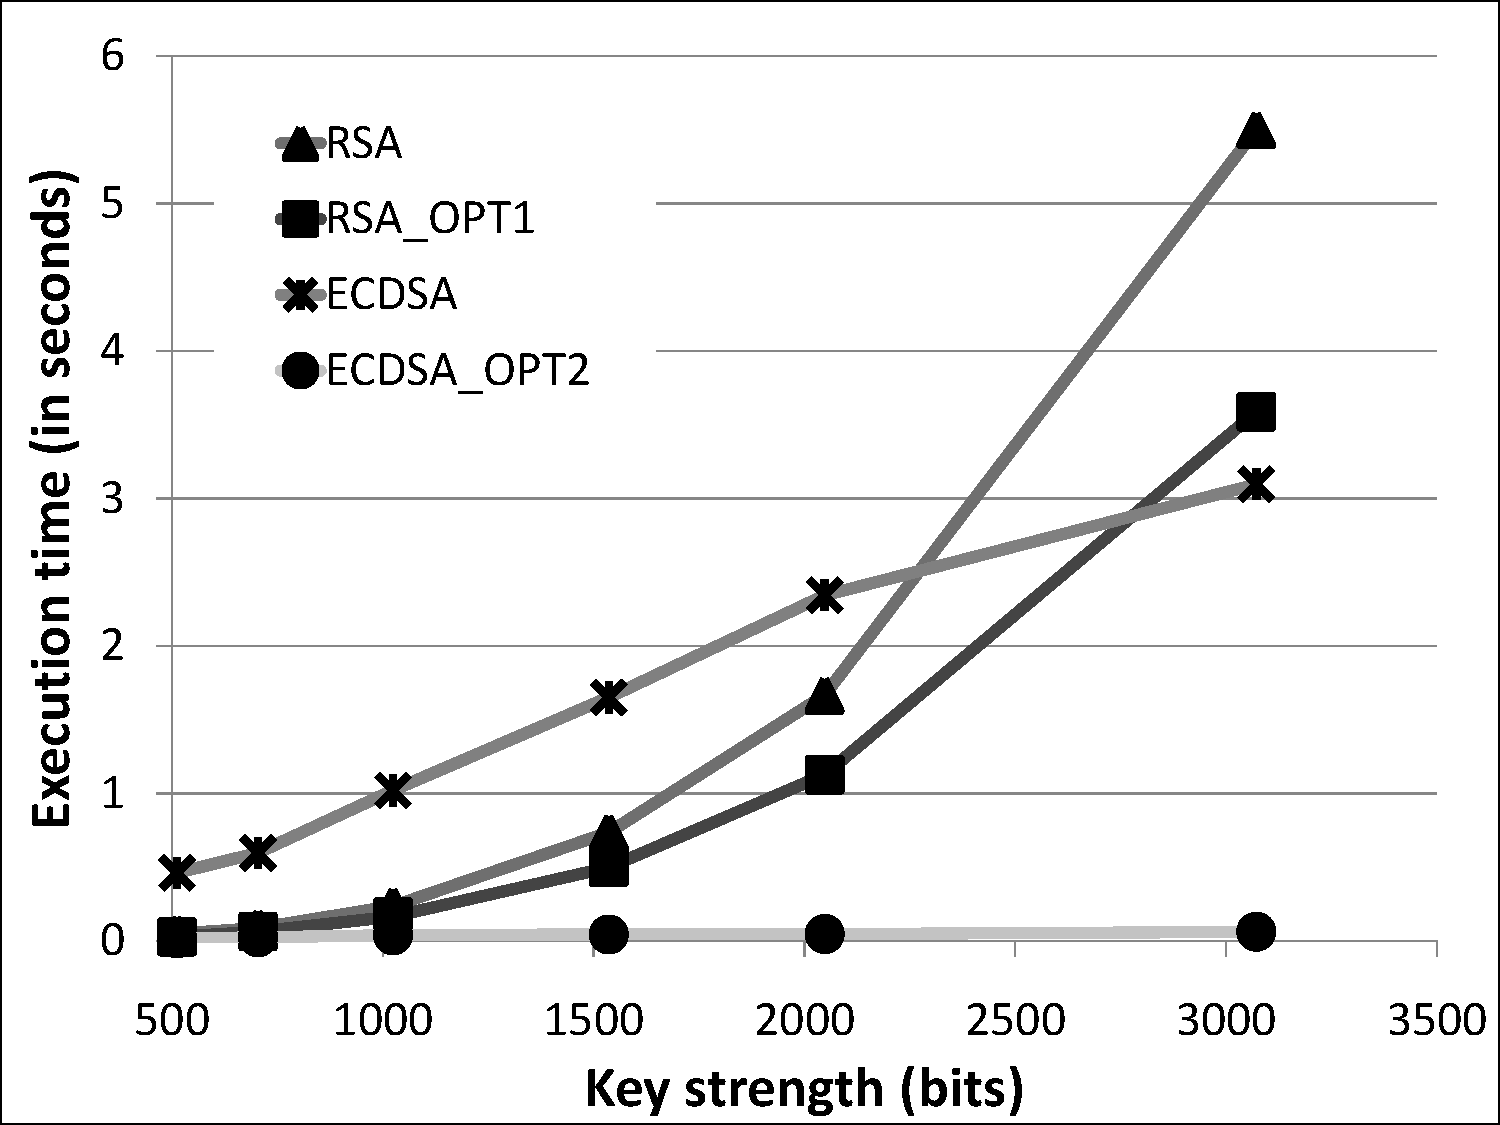
\includegraphics[width=7cm]{immagini/Firme_OPT1_OPT2.pdf}\\
  \caption{RSA and ECDSA signature generation times (in ms) on an N95-8GB device using optimizations}
  \label{fig:Firme_OPT1_OPT2}
\end{center}
\end{figure}

\begin{figure}[h]
\begin{center}
  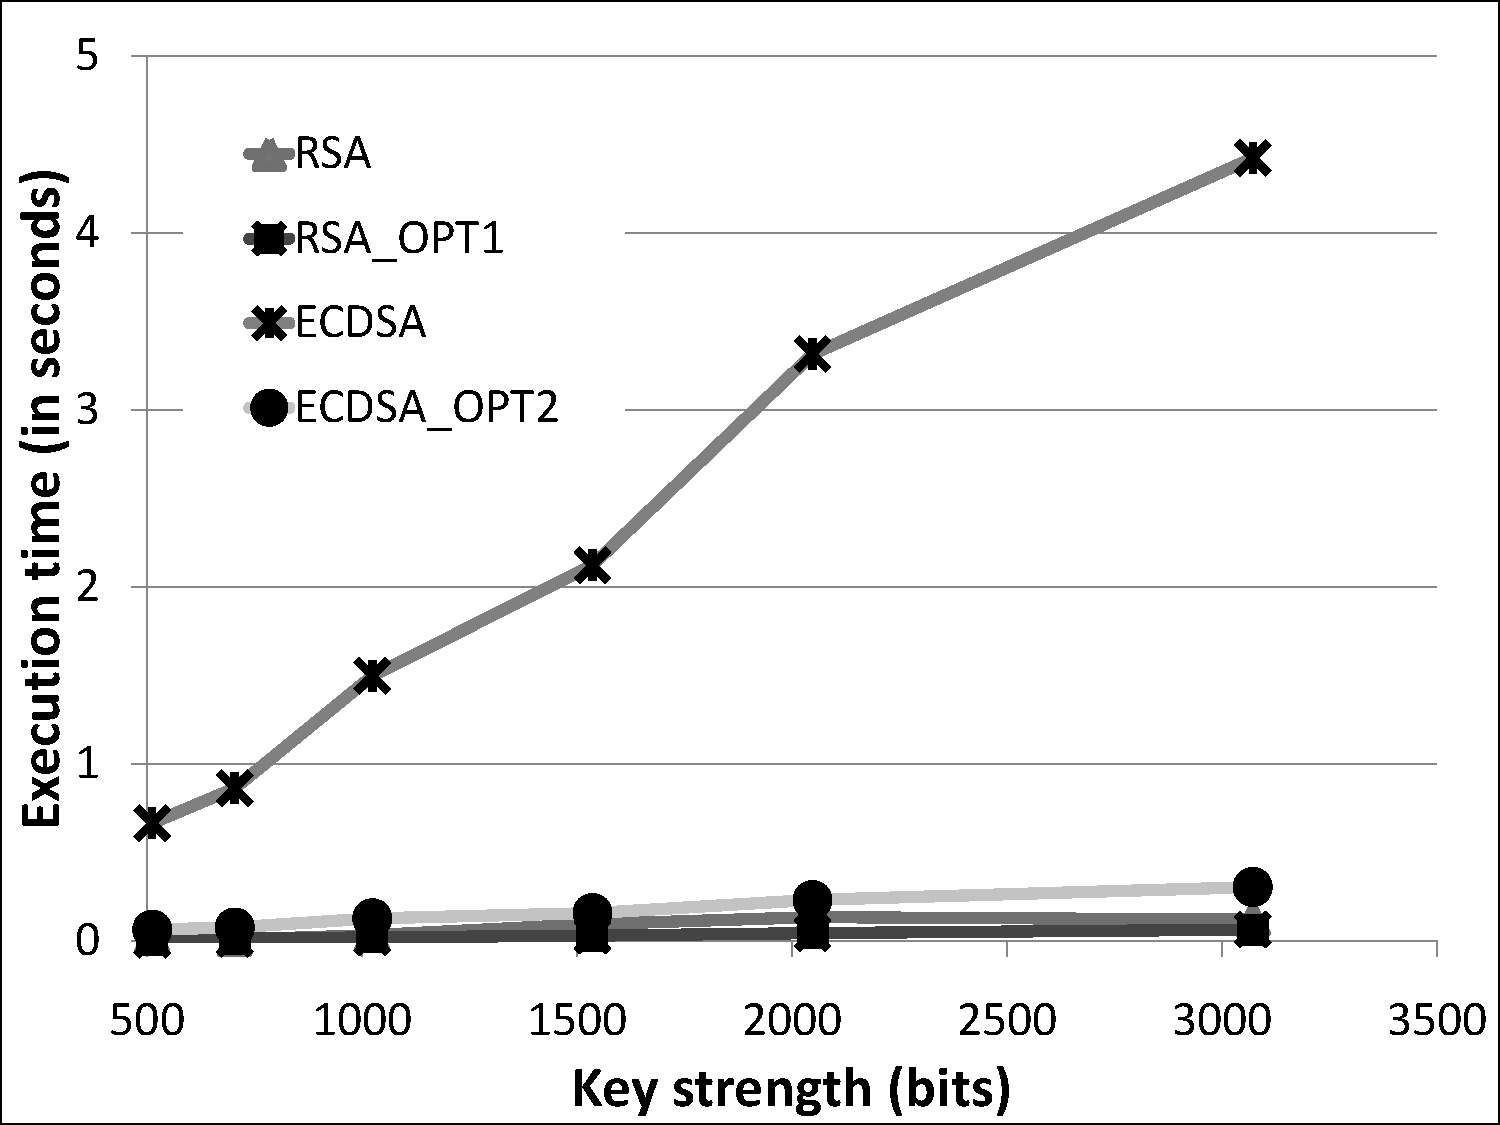
\includegraphics[width=7cm]{immagini/Verifiche_OPT1_OPT2.pdf}\\
  \caption{RSA and ECDSA signature verification times (in ms) on an N95-8GB device using optimizations}
  \label{fig:Verifiche_OPT1_OPT2}
\end{center}
\end{figure}

 

% According to the first column of Table
% \ref{table:BCJ2SE-Big_PreVSJ2SEBIG_Pre}, the result obtained by using
% precomputation contradicted the hypothesis that the ECDSA standard
% version had bad performance due to the high number of memory
% allocations that the implementation makes during the
% execution. Indeed, the version with precomputation is faster and uses
% an slightly higher number of objects (e.g., 38 curve points for curves
% over $F_p192$ are precomputed). The second column of the Table
% \ref{table:BCJ2SE-Big_PreVSJ2SEBIG_Pre} show the best result we
% obtained while improving ECDSA implementation in the Bouncy Castle
% library. It can be noticed that, with respect to the standard Bouncy
% Castle implementation without precomputation for J2ME, our
% implementation is up to 50 time faster.

% \section{Time and memory requirement for precomputation}
% We considered the time and memory required to handle the
% precomputation, verifying that technique is really usable on the
% mobile device. The precomputation consists in a vector of elliptic
% curve points. According to the Bouncy Castle implementation, each
% point is internally represented by (x,y) coordinates and curve object
% for a total of 6 elliptic curve field elements. Each field element
% consist in two big integers so we can conclude that each point need
% twelve big integers in order to be represented. Precomputation must be
% serialized in order to be saved in the filesystem and deserialized in
% order to be used. The Table \ref{table:PrecompPerf} shows, for each
% considered curve, the required precomputation size according to the
% fixed-base windowing method used and the time needed to load and
% decode the points from the filesystem on N95-8GB using J2ME and our
% big integers implementation.

% \begin{table}[ht]
% \caption{DSA and RSA signature times (in ms) on an N95-8GB device}
% \centering % used for centering table
% \begin{tabular}{|c|c|c|c|c|} % centered columns (4 columns)
% \hline\hline %inserts double horizontal lines
% Key size & DSA & DSA\_OPT1 & RSA &  RSA\_OPT1 \\
%  (bits)  & & & & \\
% %heading
% \hline\hline % inserts single horizontal line
% 512  & 78  & 29  & 49  & 27  \\
% 704  & 74  & 48  & 86  & 63  \\
% 1024 & 144 & 82  & 236 & 164 \\
% 1536 & & & 735   & 499       \\
% 2048 & & & 1666  & 1127      \\
% 3072 & & & 5503  & 3588      \\ % [1ex] adds vertical space
% \hline %inserts single line
% \end{tabular}
% \label{table:DSAVRSAJ2SEBigs} % is used to refer this table in the text
% \end{table}


\section{Conclusions}
In this paper we presented the engineering of SEESMS, a software framework that allows two peers to exchange
encrypted and digitally signed SMS  messages. A preliminary performance analysis showed that the RSA and DSA cryptosystems,
available within this framework, performed generally better than ECDSA, except when using very large keys. This conclusion seemed to contradict
the assumption on ECDSA being generally faster than RSA and justified a further investigation on the performance of the algorithmic software library we have been using.

A careful profiling of the library revealed some performance issues that were responsible for the bad performance of ECDSA. We then tried some algorithmic and programming optimization techniques for improving the performance of ECDSA. As a result of these optimizations, we obtained two variants of the original RSA and ECDSA implementations coming with the Bouncy Castle library which exhibit substantially faster execution times and a reduced memory footprint. 
Moreover, we observed faster execution times for the optimized version of ECDSA rather than RSA when signing messages, even for short keys. This experience further motivates the need for evaluating the experimental efficiency of algorithmic software libraries, prior to their adoption, in order to assess their real performance.

%
% As an additional result, we can conclude that when implementing the security features of an application, one should always accompany the choice of theoretical efficient algorithms with an experimental phase devoted to assess their practical performance, even when adopting well-known and widely used cryptographic libraries. 
% 
%
%A careful experimental analysis allowed us to pinpoint some serious performance issues that we solved by using both theoretical and programming optimization techniques.
%This experience further motivates the need for evaluating the behavior of algorithmic software libraries to assess their experimental performance 
%prior to their usage, rather than using them as black-box.




% \begin{table}[ht]
% \caption{DSA, RSA and ECDSA signature generation times (in ms) on an N95-8GB device using optimizations}
% \centering % used for centering table
% \begin{tabular}{|c|c|c|c|} % centered columns (4 columns)
% \hline\hline %inserts double horizontal lines
% Key strength & DSA\_OPT1 & RSA\_OPT1 & ECDSA\_OPT2 \\
%  (bits)  &  &  & \\
% %heading
% \hline\hline % inserts single horizontal line
% 512  & 29 & 27  & 17   \\
% 704  & 48 & 63  & 24   \\
% 1024 & 82 & 164 & 38  \\
% 1536 & & 499  & 43       \\
% 2048 & & 1127 & 46      \\
% 3072 & & 3588 & 61      \\ % [1ex] adds vertical space
% \hline %inserts single line
% \end{tabular}
% \label{table:DSAVRSAVSECDSASign} % is used to refer this table in the text
% \end{table}

% \begin{table}[ht]
% \caption{DSA, RSA and ECDSA signature verification times (in ms) on an N95-8GB device using J2SE big integers}
% \centering % used for centering table
% \begin{tabular}{|c|c|c|c|} % centered columns (4 columns)
% \hline\hline %inserts double horizontal lines
% Key strength & DSA\_OPT1 & RSA\_OPT1 & ECDSA\_OPT2 \\
%  (bits)  &  &  & \\
% %heading
% \hline\hline % inserts single horizontal line
% 512  & 69 & 6 & 63   \\
% 704  & 99 & 12 & 76   \\
% 1024 & 193 & 19 & 127  \\
% 1536 & & 30 & 157       \\
% 2048 & & 43 & 231      \\
% 3072 & & 64 & 304      \\ % [1ex] adds vertical space
% \hline %inserts single line
% \end{tabular}
% \label{table:DSAVRSAVSECDSAVerify} % is used to refer this table in the text
% \end{table}

%This behavior is likely to be due to the implementation of the ECDSA, that is probably less optimized than
% the RSA implementation available in the same library. Such explanation
% is supported also by the results of the experiments on the memory and
% power consumptions of the two algorithms, where ECDSA exhibits
% again an unexpected behavior.

% These results motivate a deeper comparative analysis of the two algorithms, focusing on the computational features of currently available mobile devices,
% and justify a further investigation on the quality of the implementation of
% the ECDSA algorithm available with the Bouncy Castle library.

% This work advises that before implementing a cryptographic application
% by using existing cryptographic libraries, it would be a good practice
% to test if the experimental performances of these libraries follow the
% expected theoretical results.

% \section{Encryption}
% We also carried on a comparative analysis on the performance of the public key encryption algorithms on mobile devices. For the encryption we tested the RSA-OAEP and the ECIES algorithm. For RSA-OAEP we expected symmetric results with respect to the RSA signature algorithm. With respect to the existing Bouncy Castle implementation, our ECIES algorithm implementation is about 20 times faster thanks to the same optimizations to the scalar multiplier which we adopted for the signature process. Tables \ref{table:Encryptiopn} and \ref{table:Decryption} show the results.

% \begin{table}[ht]
% \caption{RSA-OAEP and ECIES encryption times (in ms) on an N95-8GB device}
% \centering % used for centering table
% \begin{tabular}{|c|c|c|} % centered columns (4 columns)
% \hline\hline %inserts double horizontal lines
% Curve/ & RSA-OAEP & ECIES \\
% Key length &  J2SE-Big &  J2SE-Big + Precomp \\
% %heading
% \hline\hline % inserts single horizontal line
% secp112r2/512 & 10 & 128 \\
% secp128r2/704 & 14 & 145 \\
% secp160r2/1024 & 9 & 187 \\
% secp192r1/1536 & 13 & 219 \\
% secp224r1/2048 & 20 & 251 \\
% secp256r1/3072 & 37 & 289 \\
% \hline %inserts single line
% \end{tabular}
% \label{table:Encryptiopn} % is used to refer this table in the text
% \end{table}

% \begin{table}[ht]
% \caption{RSA-OAEP and ECIES decryption times (in ms) on an N95-8GB device}
% \centering % used for centering table
% \begin{tabular}{|c|c|c|} % centered columns (4 columns)
% \hline\hline %inserts double horizontal lines
% Curve/ & RSA-OAEP & ECIES \\
% Key length &  J2SE-Big &  J2SE-Big + Precomp \\
% %heading
% \hline\hline % inserts single horizontal line
% secp112r2/512 & 29 & 171 \\
% secp128r2/704 & 69 & 211 \\
% secp160r2/1024 & 166 & 354 \\
% secp192r1/1536 & 501 & 513 \\
% secp224r1/2048 & 1164 & 704 \\
% secp256r1/3072 & 3648 & 1135 \\
% \hline %inserts single line
% \end{tabular}
% \label{table:Decryption} % is used to refer this table in the text
% \end{table}

% This paper presents SEESMS, a software framework that allows
% two peers to exchange encrypted and digitally signed SMS
% messages. SEESMS differs from the other frameworks presented so far
% in literature, because it allows users to choose which cryptosystem and
% which degree of security to use. Three cryptosystems are built-in, RSA, DSA
% and ECDSA and further can be added thanks to his modular architecture.
% An experimental analysis of the cryptosystems available in SEESMS
% using several different metrics have been conducted.

% The results seem to show that RSA and DSA cryptosystems perform generally better than ECDSA, except when using very large keys. This conclusion contradicts the assumption on ECDSA being generally faster than RSA. This behavior is likely to be due to the implementation of the ECDSA, that is probably less optimized than
% the RSA implementation available in the same library. Such explanation
% is supported also by the results of the experiments on the memory and
% power consumptions of the two algorithms, where ECDSA exhibits
% again an unexpected behavior.

% These results motivate a deeper comparative analysis of the two algorithms, focusing on the computational features of currently available mobile devices,
% and justify a further investigation on the quality of the implementation of
% the ECDSA algorithm available with the Bouncy Castle library.

%\begin{table}[ht]
%\caption{EC precomputation size (in bytes) and the time to load it from store on N95-8GB }
%\centering % used for centering table
%\begin{tabular}{|c|c|c|c|} % centered columns (4 columns)
%\hline\hline %inserts double horizontal lines
%Curves & Size & Loading time & Loading time \\
%  &  &  & using J2SE-Big \\
%%heading
%\hline\hline % inserts single horizontal line
%secp112r2 & 471 & 205 & 232   \\
%secp128r2 & 499 & 440 & 292    \\
%secp160r2 & 763 & 527 & 391   \\
%secp192r1 & 1056 & 787 & 425   \\
%secp224r1 & 1398 & 1060 & 720   \\
%secp256r1 & 1821 & 1365 & 995   \\ % [1ex] adds vertical space
%\hline %inserts single line
%\end{tabular}
%\label{table:PrecompPerf} % is used to refer this table in the text
%\end{table}
\begin{figure}[h]
\begin{center}
  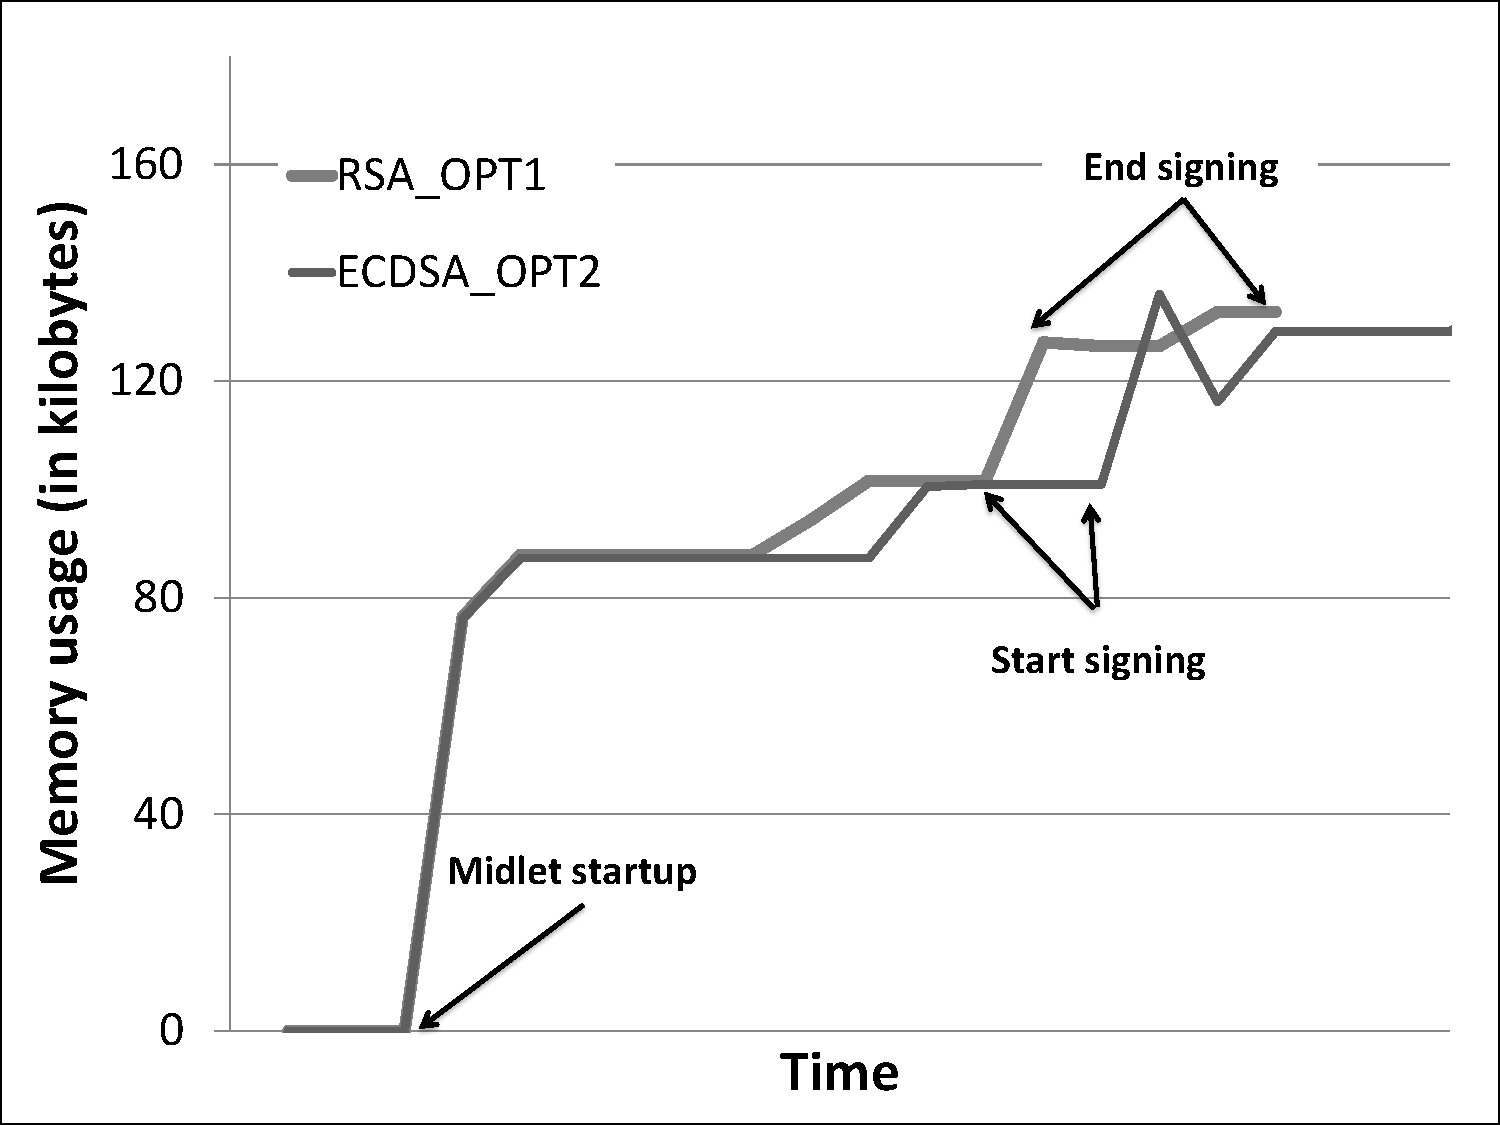
\includegraphics[width=6.8cm]{immagini/MemoryRSA1ECDSA2.pdf}\\
  \caption{Memory usage profile of \textbf{RSA\_OPT1} and \textbf{ECDSA\_OPT2} when processing a 1024-bit and a 160-bit signature respectively}
  \label{fig:MemoryRSA1ECDSA2}
\end{center}
\end{figure}

\newpage


\begin{figure}[t]
\begin{center}
  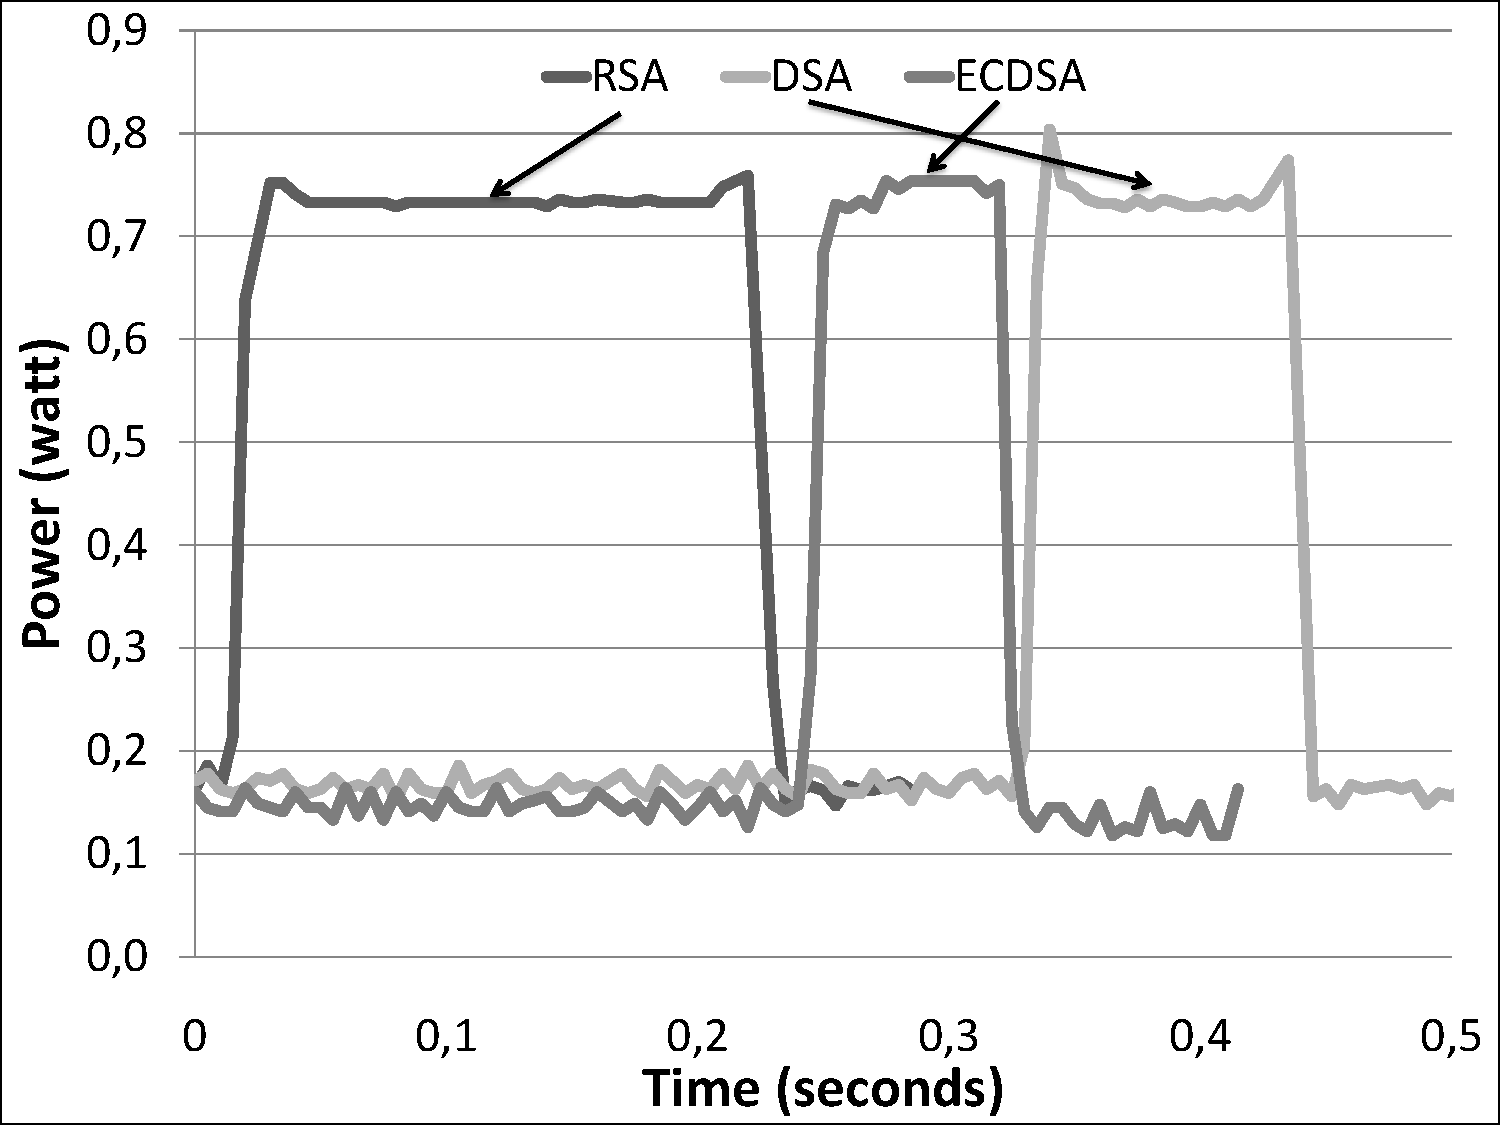
\includegraphics[width=7cm]{immagini/Power_OPT.pdf}\\
  \caption{N95-8GB power consumption when signing a message using a $1.024$ bits key using optimized algorithm and implementation}
  \label{fig:N95Power_OPT}
\end{center}
\end{figure}


\begin{figure}[h.q.]
\begin{center}
  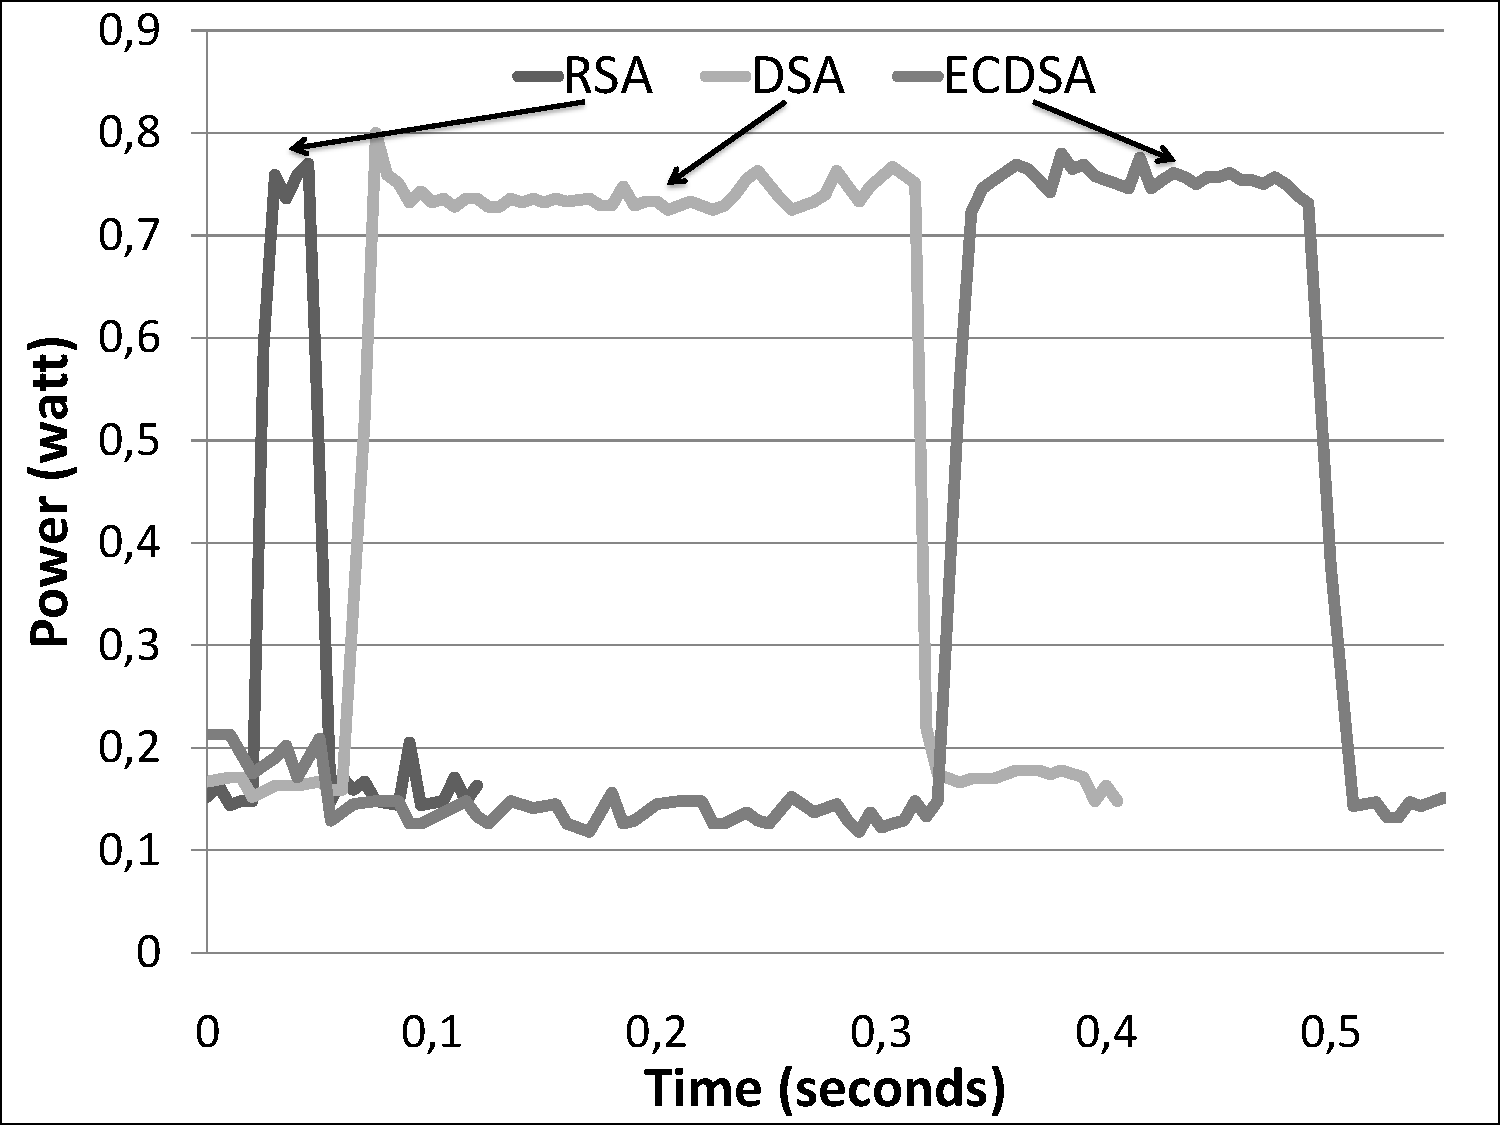
\includegraphics[width=7cm]{immagini/N95PowerVerify_OPT.pdf}\\
  \caption{N95-8GB power consumption when verifying a message using a $1.024$ bits key using optimized algorithm and implementation}
  \label{fig:N95PowerVerify_OPT}
\end{center}
\end{figure}

%\bibliographystyle{model2-names}
\bibliographystyle{elsarticle-harv}
%\balance
\bibliography{SEESMS_journal}

\newpage

\textbf{Aniello Castiglione} joined the Dipartimento di Informatica ed Applicazioni ``R. M. Capocelli" of Universit\'{a} di Salerno in February 2006. He received a degree in Computer Science and his Ph.D. in Computer Science from the same university.
He is a reviewer for several international journals (Elsevier, Hindawi, IEEE, Springer) and he has been a member of international conference committees. He is a Member of various associations, including: IEEE (Institute of Electrical and Electronics Engineers), of ACM (Association for Computing Machinery), of IEEE Computer Society, of IEEE Communications Society, of GRIN (Gruppo di Informatica) and of  IISFA (International Information System Forensics Association, Italian Chapter). He is a Fellow of FSF (Free Software Foundation) as well as FSFE (Free Software Foundation Europe). For many years, he has been involved in forensic investigations, collaborating with several Law Enforcement agencies as a consultant. His research interests include Data Security, Communication Networks, Digital Forensics, Computer Forensics, Security and Privacy, Security Standards and Cryptography.

\medskip

\textbf{Giuseppe Cattaneo} received a degree in Computer Science from the Universit\`a di Salerno in 1983.
Since 1986 he has been research associate with the Dipartimento di Informatica ed Applicazioni
where he is actually working as associate professor. From 1987 to 1990 he has been visiting researcher at LITP (Laboratoire d'Informatique Th\'eorique et Programmation) of the  Universit\'e Paris 6 working on a project aimed to the development of a Parallel Lisp Machine designing and implementing special purpose extensions to the functional language dedicated to the explicit parallelism management. Since 1993 he approached to System Security and particularly experimental algorithm evaluation and algorithm engineering. In the last 10 years he has been team leader and responsible of the local unit of 8 ICT projects co-funded by national large companies.

\medskip
\textbf{Maurizio Cembalo} was born in Naples in 1982. He received a master degree in Computer Science (cum laude) in 2007 and his PhD in Computer Science in 2011 from the Universit\'{a} di Salerno. His research interests include Security and Privacy, Applied Crypthograghy, Mobile device security and Image Forensic.


\medskip

\textbf{Alfredo De Santis} received a degree in Computer Science (cum laude) from the Universit\'{a} di Salerno in 1983. Since 1984, he has been with the Dipartimento di Informatica ed Applicazioni of the Universit\'{a} di Salerno. Since 1990 he is a Professor of Computer Science. From November 1991 to October 1995 and from November 1998 to October 2001 he was the Chairman of the Dipartimento di Informatica ed Applicazioni, Universit\'{a} di Salerno. From November 1996 to October 2003 he was the Chairman of the PhD Program in Computer Science at the Universit\'{a} di Salerno. From September 1987 to February 1990 he was a Visiting Scientist at IBM T. J. Watson Research Center, Yorktown Heights, New York. He spent August 1994 at the International Computer Science Institute (ICSI), Berkeley CA, USA, as a Visiting Scientist. From November 2009 he is in the Board of Directors of Consortium GARR (the Italian Academic \& Research Network). His research interests include Algorithms, Data Security, Cryptography, Information Forensics, Communication Networks, Information Theory, and Data Compression.

\medskip

\textbf{Pompeo Faruolo} was born in Salerno in 1975. He got his Laurea
(M.Sc. equivalent) cum laude in Computer Science in 2001 and his PhD
in Computer Science in 2005 from the Universit\'{a} di Salerno. Currently,
he is a Post-Doctoral fellow at the Universit\'{a} di Salerno. His
research interests include Algorithm Engineering, Distributed Systems
and Network Security.

\medskip

\textbf{Umberto Ferraro Petrillo} is currently an assistant professor
in Computer Science at the Dipartimento of Scienze
Statistiche of Universit\'{a} di Roma - ``Sapienza". He got his Laurea (M.Sc. equivalent) cum laude in
Computer Science in 1997 and his PhD in Computer Science in 2002 from
the Universit\'{a} di Salerno. He has been a Post-Doctoral fellow in Roma
at the Institute for Industrial Technologies and Applications of the
Italian National Research Council (from January to April 2002) and at
Universit\'{a} di Roma - "Tor Vergata" (from May to September 2002), at the
Universit\'{a} di Salerno (from September 2002 to September 2004) and, finally, at
the Universit\'{a} di Roma - ``Sapienza" (from January 2005 to November 2006).

He is senior researcher on the topics related to the development and
the experimentation of Efficient Algorithms such as algorithms for
maintaining properties on graphs subject to structural changes,
algorithms for the packed sorting and algorithms for sorting and
searching efficiently in presence of memory faults.  His research
interests include also Security on Communication Networks and Software
Visualization.

\medskip

\textbf{Fabio Petagna} is a PhD student in Computer Science at the Universit\'{a} di Salerno. He got his Laurea
(M.Sc. equivalent) in Computer Science in 2005 from the Universit\'{a} di Salerno and from November 2007, and his PhD in Computer Science in 2011 from the Universit\'{a} di Salerno. His research interests include Network Protocols, Communication Networks, Security and Privacy, Applied Cryptography, VoIP and Mobile Devices Security.


\end{document}
